\chapter{Методика работы} \label{chapt3}

\section{Критерии отбора данных и подготовка данных к физическому анализу} \label{sect3_cuts}
В данной работе были использованы данные, полученные экспериментом PHENIX, в столкновениях $p+p$ (2005 год набора данных, доставленная интегральная светимость $L=29.5$ пб$^{-1}$), Cu+Au (2012 г., $L=27.0$ нб$^{-1}$), U+U (2012 г., $L=736$ мкб$^{-1}$), \heau \ (2014 г., $L=134$ нб$^{-1}$) и $p$+Al (2015 г., $L=3.87$ пб$^{-1}$).


\begin{table}
	\caption{Критерии отбора данных}
	\centerfloat{\begin{tabular}{|c|c|}
		\hline
	 
		%Показатель качества треков & $31||63||51$ \\ \hline
		% & $|zed| < $ 75 cm \& $|zed|>$ 4 cm \\ \hline
		\multicolumn{2}{|c|}{\pal \ столкновения при \sqsn \ = 200 ГэВ: $\sim$2$\cdot 10^9$ событий}\\ 
		\multicolumn{2}{|c|}{\heau \ столкновения при \sqsn \ = 200 ГэВ: $\sim$2,8$\cdot 10^9$ событий}\\ 
		\multicolumn{2}{|c|}{Cu+Au столкновения при \sqsn \ = 200 ГэВ: $\sim$7$\cdot 10^9$ событий}\\ 
		\multicolumn{2}{|c|}{U+U столкновения при \sqsn \ = 193 ГэВ: $\sim$1,2$\cdot 10^9$ событий}\\ \hline
		Ограничение $z$-координаты & \multirow{2}{*}{$|z_{vtx}| < $ 30 см} \\ % \cline{1-1}
		вершины столкновения    &          \\ \hline
		Биты качества отслеживания  &  31 || 63 || 51   \\ 
		($Q_{track}$)  &    \\ \hline
		Ограничение величины $zed$  &  4 см < $|zed|$ < 75 см  \\ \hline
		\multirow{4}{*}{Интервал \pt \ измерения \pipm} & \pal \ -- 0,5 ГэВ/$c$ $< p_T < $ 2,0 ГэВ/$c$ \\
		& \heau \ -- 0,5 ГэВ/$c$ $< p_T < $ 3,0 ГэВ/$c$  \\ 
		& \cuau \ -- 0,5 ГэВ/$c$ $< p_T < $ 3,0 ГэВ/$c$  \\ 
		& \uu \ -- 0,5 ГэВ/$c$ $< p_T < $ 3,5 ГэВ/$c$  \\ \hline
			\multirow{4}{*}{Интервал \pt \ измерения \Kpm} & \pal \ -- 0,5 ГэВ/$c$ $< p_T < $ 1,8 ГэВ/$c$ \\
		& \heau \ -- 0,5 ГэВ/$c$ $< p_T < $ 2,0 ГэВ/$c$  \\ 
		& \cuau \ -- 0,5 ГэВ/$c$ $< p_T < $ 2,0 ГэВ/$c$  \\ 
		& \uu \ -- 0,5 ГэВ/$c$ $< p_T < $ 2,0 ГэВ/$c$  \\ \hline
		\multirow{4}{*}{Интервал \pt  \ измерения \prot \ и \aprot} & \pal \ -- 0,5 ГэВ/$c$ $< p_T < $ 2,5 ГэВ/$c$ \\
		& \heau \ -- 0,5 ГэВ/$c$ $< p_T < $ 4,0 ГэВ/$c$  \\ 
		& \cuau \ -- 0,5 ГэВ/$c$ $< p_T < $ 4,0 ГэВ/$c$  \\ 
		& \uu \ -- 0,5 ГэВ/$c$ $< p_T < $ 4,0 ГэВ/$c$  \\ \hline
			
	\end{tabular}}
	\label{table:cuts}
\end{table}

Критерии отбора данных, использованные в анализе, приведены в Таблице \ref{table:cuts}. Выбор событий с минимальным отбором, ограничения $z$-координаты вершины столкновения $z_{vtx}$ и величины $|zed|$, а также выбор бита качества отслеживания являются общепринятыми критериями в эксперименте PHENIX. Также в данной работе были использованы специфические критерии отбора данных -- критерии идентификации заряженных частиц с использованием дрейфовой камеры и времяпролетных детекторов. Критерии идентификации заряженных частиц рассмотрены в Разделе \ref{sect3_PID}.

Приведенные критерии отбора данных были также использованы при Монте-Карло моделировании, которое проводилось для оценки эффективности регистрации частиц (см. Раздел \ref{sect3:EffRec}) и коррекции, учитывающей увеличение выхода протонов и антипротонов в результате распада частиц (см. Раздел \ref{sect3:FeedDown}). 

\subsection{Триггер минимального отбора}
В качестве основного набора данных в эксперименте PHENIX используется набор данных с минимальным отбором (<<Minimum Bias>> -- MB), который формируется с помощью триггера минимального отбора (MB-триггера).
MB-триггер отбирает события, в которых происходит одновременное срабатывание двух или более ФЭУ из состава BBC счетчиков, расположенных в северном плече эксперимента PHENIX (передняя область быстрот) и южном плече эксперимента PHENIX (задняя область быстрот).
Также события минимального отбора должны удовлетворять условию на ограничение $z$-координаты вершины столкновения $|z_{vtx}| < $ 30 см. Отбор данных событий осуществляется онлайн с помощью триггера BBC первого уровня LVL1.

Эффективность MB-триггера определяется с помощью Монте-Карло моделирования BBC. Отклик ФЭУ и логика платы BBLL1 настраиваются при моделировании в соответствии с условиями эксперимента. Эффективность триггера для неупругих столкновений A+B составляет 92 ± 2\%. 

Поскольку MB-триггер расположен вблизи оси пучка, эффективность регистрации дифракционных событий оказывается выше, чем недифракционных, поскольку для дифракционных событий характерны большие множественности рождения частиц в диапазонах по быстроте $3 <|y|<4$, в то время как недифракционные события характеризуются рождением частиц преимущественно в области малых быстрот $|y|<0,35$. Зависимость эффективности MB-триггера от множественности события в области больших быстрот корректируется с помощью Байес-фактора ($f_{Bias}$). 
Значения поправок $f_{Bias}$ были оценены с помощью моделирования МК Глаубера и представлены в Таблице \ref{table:fBias}.

\begin{table}[]
	\caption{Значения $f_{Bias}$, вычисленные с помощью модели Глаубера для различных центральностей \pal \ и \heau \ столкновений.}
	\label{table:fBias}
	
	\begin{tabularx}{\linewidth}
		{
			| >{\centering\arraybackslash}X
			| >{\centering\arraybackslash}X
			| >{\centering\arraybackslash}X | }
		\hline
		Система столкновения & Центральность &  $f_{bias}$  \\ \hline
		\pal & 0-72\%     & 0,80$\pm$0,02       \\
		& 0-20\%     & 0,81$\pm$0,01       \\
		& 20-40\%    & 0,90$\pm$0,02       \\
		& 40-72\%    & 1,05$\pm$0,04    \\ \hline
		
		\heau & 0-88\%     & 0,89$\pm$0,01  \\
		& 0-20\%     & 0,95$\pm$0,01  \\
		& 20-40\%    & 1,01$\pm$0,01  \\
		& 40-60\%    & 1,02$\pm$0,01   \\
		& 60-88\%    & 1,03$\pm$0,05   \\ \hline
		
	\end{tabularx}
\end{table}

\subsection{Определение центральности} \label{sect3:centr}
Центральность является характеристикой столкновения, показывающей степень перекрытия ядер, и непосредственно связанна с прицельным параметром. Лобовым столкновениям с прицельным параметром равным нулю, в которых степень перекрытия ядер максимальна, соответствует значение центральности 0\%. Периферическим столкновениям, в которых ядра проходят по касательной, а прицельный параметр равен сумме радиусов сталкивающихся ядер, соответствует значение центральности 100 \%. В остальных случаях значения центральности варьируются от 0\% до 100 \%, характеризуя степень перекрытия ядер.


\begin{figure}[] 
	\centerfloat
	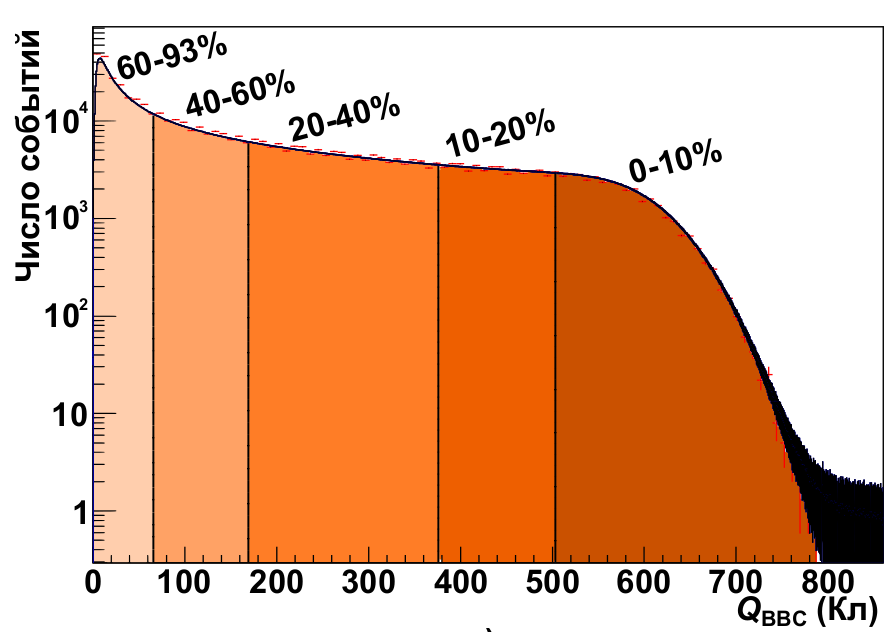
\includegraphics [width=0.7\linewidth]{Methodology/centrality.png}
	\caption{Распределение событий Cu+Au столкновений по величине заряда, зарегистрированного в счетчиках BBC} 
	\label{img:Met_centr}
\end{figure}

Центральность столкновения в эксперименте PHENIX определяется с помощью BBС детектора, который измеряет количество заряженных частиц в переднем и заднем диапазоне быстрот ($3<|\eta|<4$). 
Для определения центральности заполняется гистограмма распределения событий ядро-ядерных столкновений по величине заряда, зарегистрированного в BBC счетчике. Пример данной гистограммы для Cu+Au столкновений приведен на Рисунке \ref{img:Met_centr}. Далее полученная гистограмма разбивается на части, количество событий в которых пропорционально рассматриваемым интервалам центральности. Разбиение, соответствующее интервалам центральности 0–20 \%, 20–40 \%, 40–60 \%, 60–82 \% обозначено на графике линиями. Интервал центральности 60-92 \% используется как самый периферийный в связи с низкой статистикой в периферических столкновениях.



\begin{table}[]
	\caption{Значения \Ncoll \ и \Npart, вычисленные с помощью модели Глаубера для различных центральностей \pal, \heau, \cuau \ и \uu \ столкновений.}
	\label{table:NcollNpart}
	
	\begin{tabularx}{\linewidth}
		{
			| >{\centering\arraybackslash}X
			| >{\centering\arraybackslash}X
			| >{\centering\arraybackslash}X | }
		\hline
			Центральность & \Ncoll    &  \Npart       \\ \hline  \hline
			\multicolumn{3}{|c|}{\pal}\\ \hline
			0-72\%     & 2,1$\pm$0,2    & 3,1$\pm$0,1    \\  \hline
			0-20\%     & 3,4$\pm$0,3    & 4,4$\pm$0,3    \\ \hline
			20-40\%    & 2,3$\pm$0,2    & 3,3$\pm$0,1    \\ \hline
			40-72\%    & 1,7$\pm$0,1   & 1,6$\pm$0,2  \\ \hline  \hline
     		\multicolumn{3}{|c|}{\heau}\\ \hline	
			0-88\%     & 10,4$\pm$0,7 & 11,3$\pm$0,5    \\  \hline
			0-20\%     & 22,3$\pm$1,7 & 21,1$\pm$1,3    \\ \hline
			20-40\%    & 14,8$\pm$1,1 & 15,4$\pm$0,9    \\ \hline
			40-60\%    & 8,4$\pm$0,6  & 9,5$\pm$0,6     \\ \hline
			0-88\%    & 3,4$\pm$0,3  & 4,8$\pm$0,3     \\  \hline  \hline
      		\multicolumn{3}{|c|}{Cu+Au}\\ \hline
			0-80\%     & 123,8$\pm$12,0  & 70,4$\pm$3,0    \\  \hline
			0-20\%     & 313,8$\pm$28,4  & 154,8$\pm$4,1     \\  \hline
			20-40\%    & 129,3$\pm$12,4  & 80,4$\pm$3,3     \\  \hline
			40-60\%    & 41,8$\pm$5,3    & 34,9$\pm$2,9   \\ \hline
			60-80\%    & 10,1$\pm$2,0    & 11,5$\pm$1,8   \\ \hline  \hline
      		\multicolumn{3}{|c|}{U+U}\\ \hline
			0-20\%     & 935$\pm$98    & 330$\pm$6   \\ \hline
			20-40\%    & 335$\pm$33    & 259$\pm$7   \\ \hline
			40-60\%    & 81$\pm$13     & 65$\pm$6    \\ \hline
			60-80\%    & 17$\pm$4  & 18$\pm$3   \\
				\hline
	
	\end{tabularx}
\end{table}

Центральность столкновения связана с величинами $N_{part}$ и $N_{coll}$ - количеством нуклонов участников и количеством парных нуклон-нуклонных соударений соответственно. Величины $N_{part}$ и $N_{coll}$ были определены с помощью модели Глаубера и представлены в Таблице \ref{table:NcollNpart}.

\subsection{Исключение проблемных сегментов} \label{sect3_DM}
За время эксплуатации эксперимента PHENIX некоторые сегменты дрейфовых камер выходят из строя, что приводит к уменьшению уровня загрузки ДК. Области низкой загрузки ДК принято называть <<мертвыми>> областями. 
Для корректной оценки эффективности регистрации заряженных адронов необходимо исключить мертвые области из дальнейшего анализа. 
Исключение мертвых областей проводится с помощью построения гистограмм загрузки ДК, которые представляют собой распределение уровня загрузки дрейфовой камеры в зависимости от угла $\alpha$ и полярного угла $\varphi$, который для удобства заменяется номером <<платы>>. Номер <<платы>> $N$ связан с углом $\varphi$ треков заряженных частиц следующими соотношениями: 

\begin{equation}
	N_{восточное плечо} = \left( \frac{3,72402 - \varphi + 0,008047 \cdot cos(\varphi + 0,87851)}{0,01963496} \right),
\end{equation}


\begin{equation}
	N_{западное плечо} = \left( \frac{0,573231 + \varphi - 0,0046 \cdot cos(\varphi + 0,05721)}{0,01963496} \right).
\end{equation}

Полученные гистограммы загрузки представлены на Рисунках \ref{img:Met_DMRun12}-\ref{img:Met_DMRun15}. 
На гистограммах загрузки ДК (панели а), в) на Рисунках \ref{img:Met_DMRun12}-\ref{img:Met_DMRun15}) присутствуют <<мертвые>> области, уровень загрузки в которых значительно ниже среднего по камере. 
%Такие области дрейфовых камер с пониженной загрузкой  принято называть <<мертвыми>> областями. 
%Для уменьшения искажений мертвые области исключаются из анализа.
Панели б), г) на Рисунках \ref{img:Met_DMRun12}-\ref{img:Met_DMRun15} представляют гистограмму загрузки ДК после исключения мертвых областей. 
Совокупность мертвых областей, исключаемых из анализа, называется мертвой картой дрейфовой камеры. Мертвые карты также были применены при проведении моделирования (см. Раздел \ref{sect3:EffRec}).


\begin{figure}[] 
	\centerfloat
	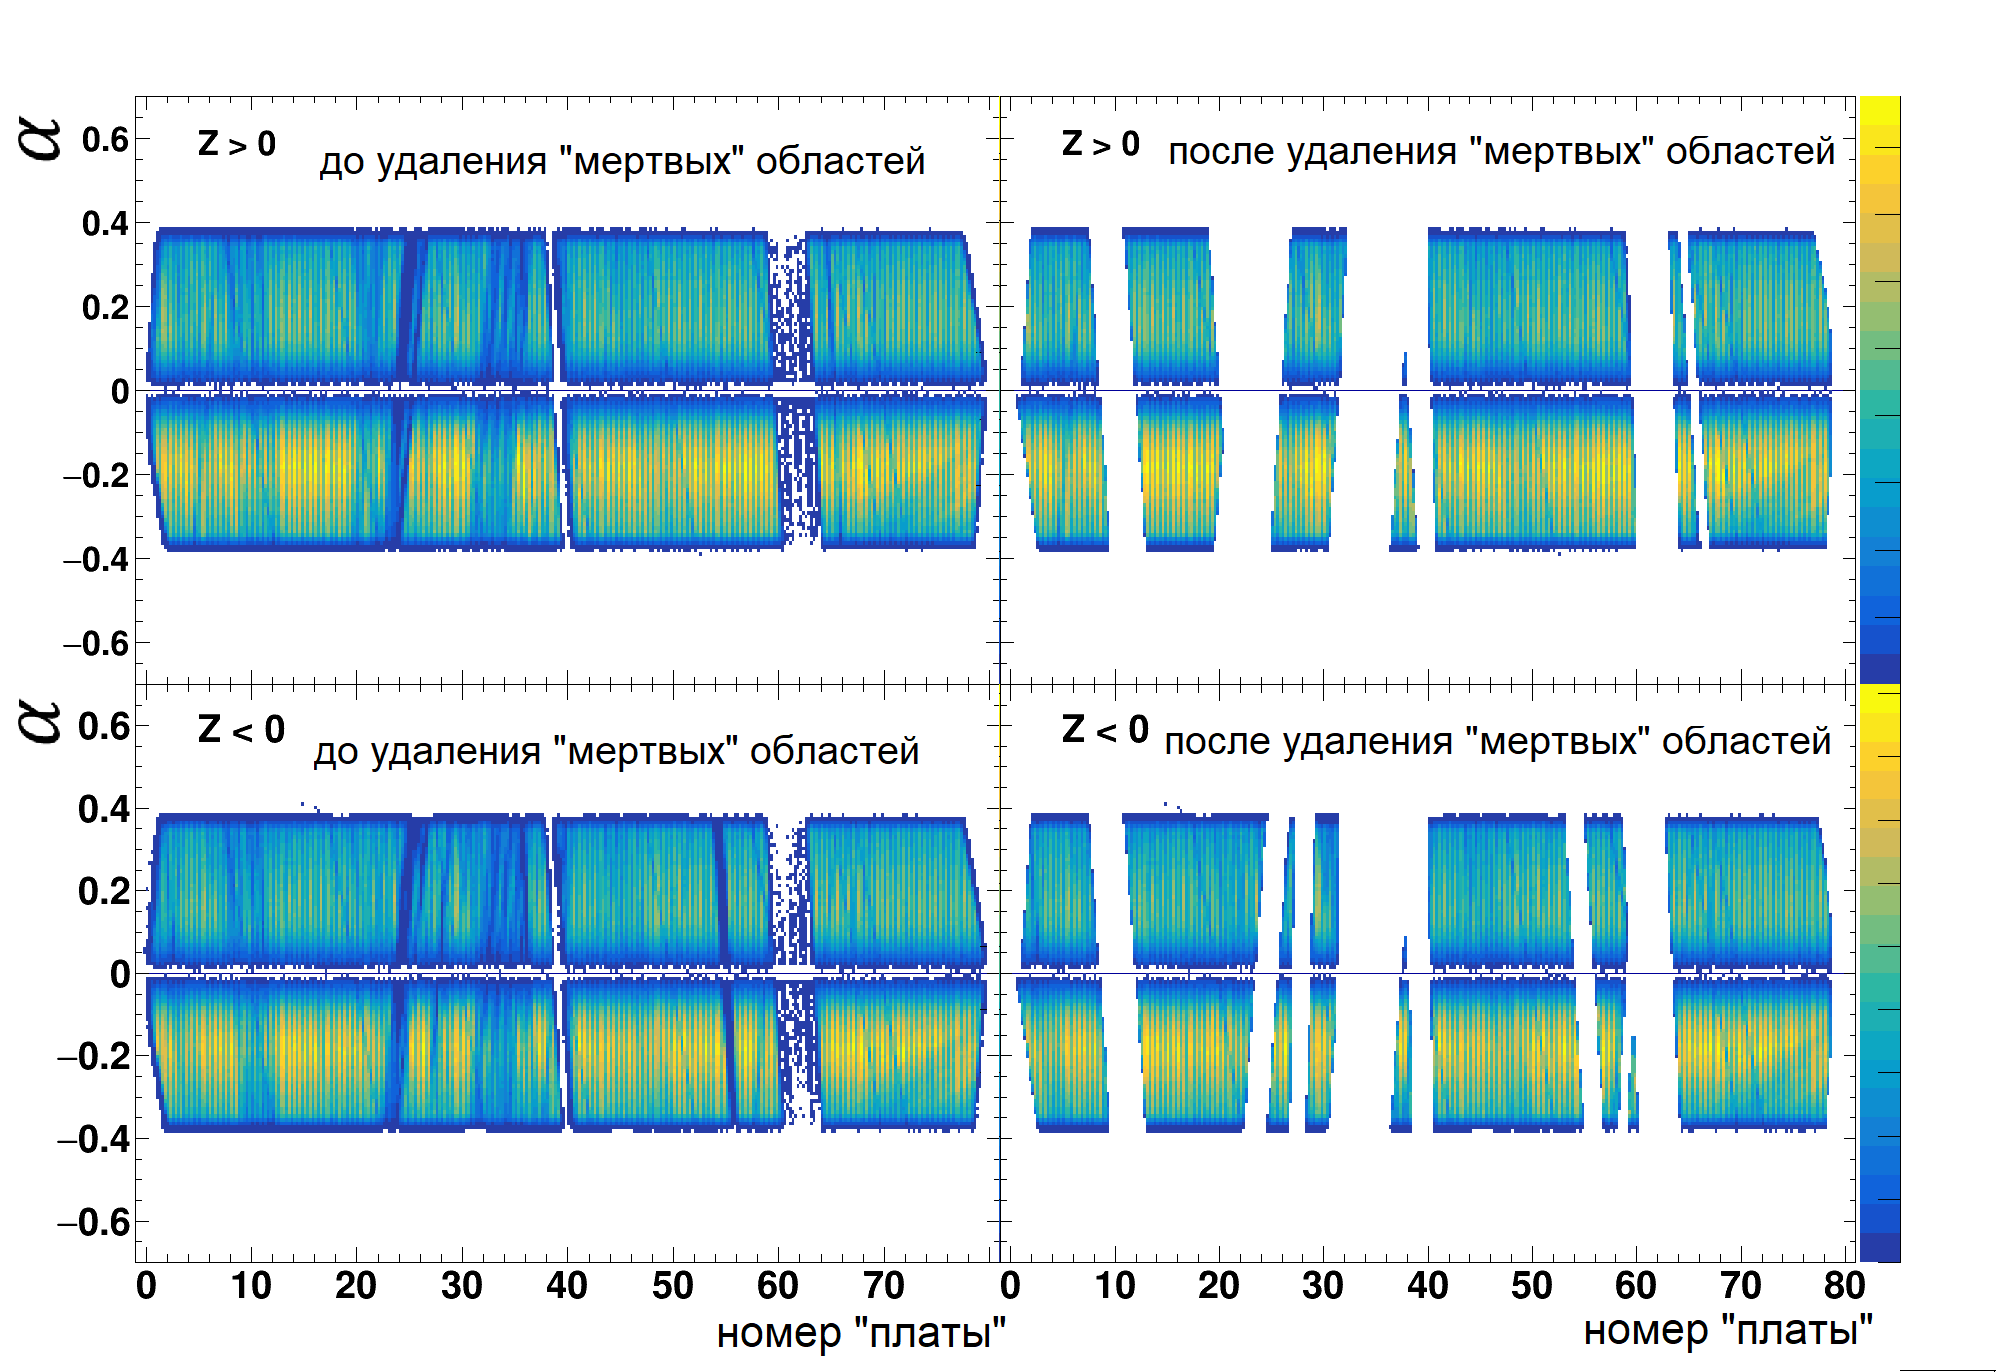
\includegraphics [width=0.8\linewidth]{Methodology/DC_DM_HeAu.png}
	\caption{Гистограмма загрузки дрейфовых камер в 2012 году} 
	\label{img:Met_DMRun12}
\end{figure}

\begin{figure}[] 
	\centerfloat
	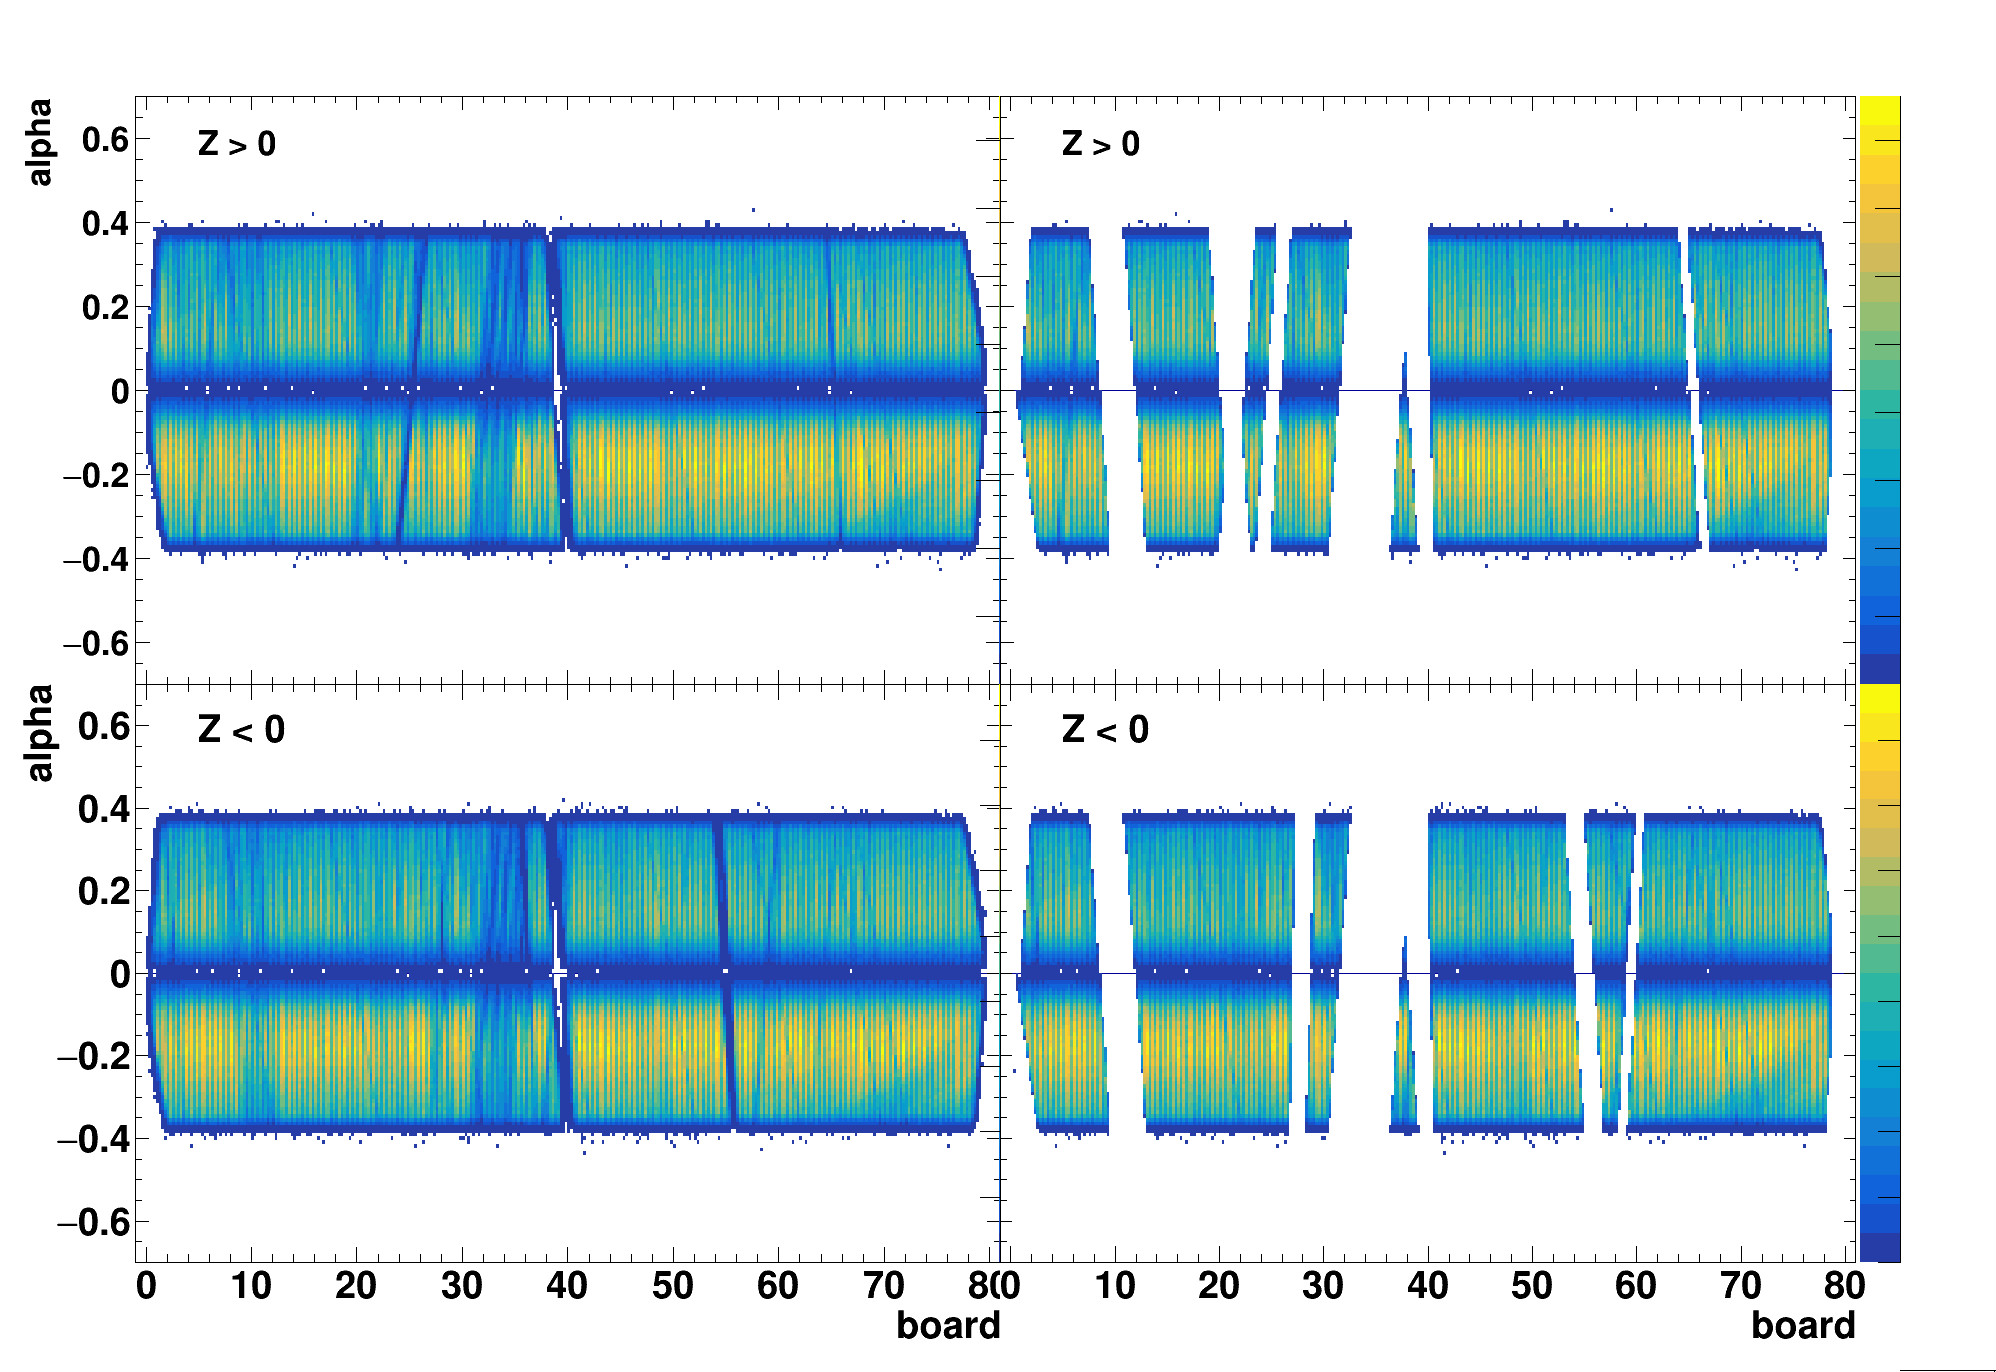
\includegraphics [width=0.8\linewidth]{Methodology/DC_DM_CuAu.png}
	\caption{Гистограмма загрузки дрейфовых камер в 2014 году} 
	\label{img:Met_DMRun14}
\end{figure}

\begin{figure}[] 
	\centerfloat
	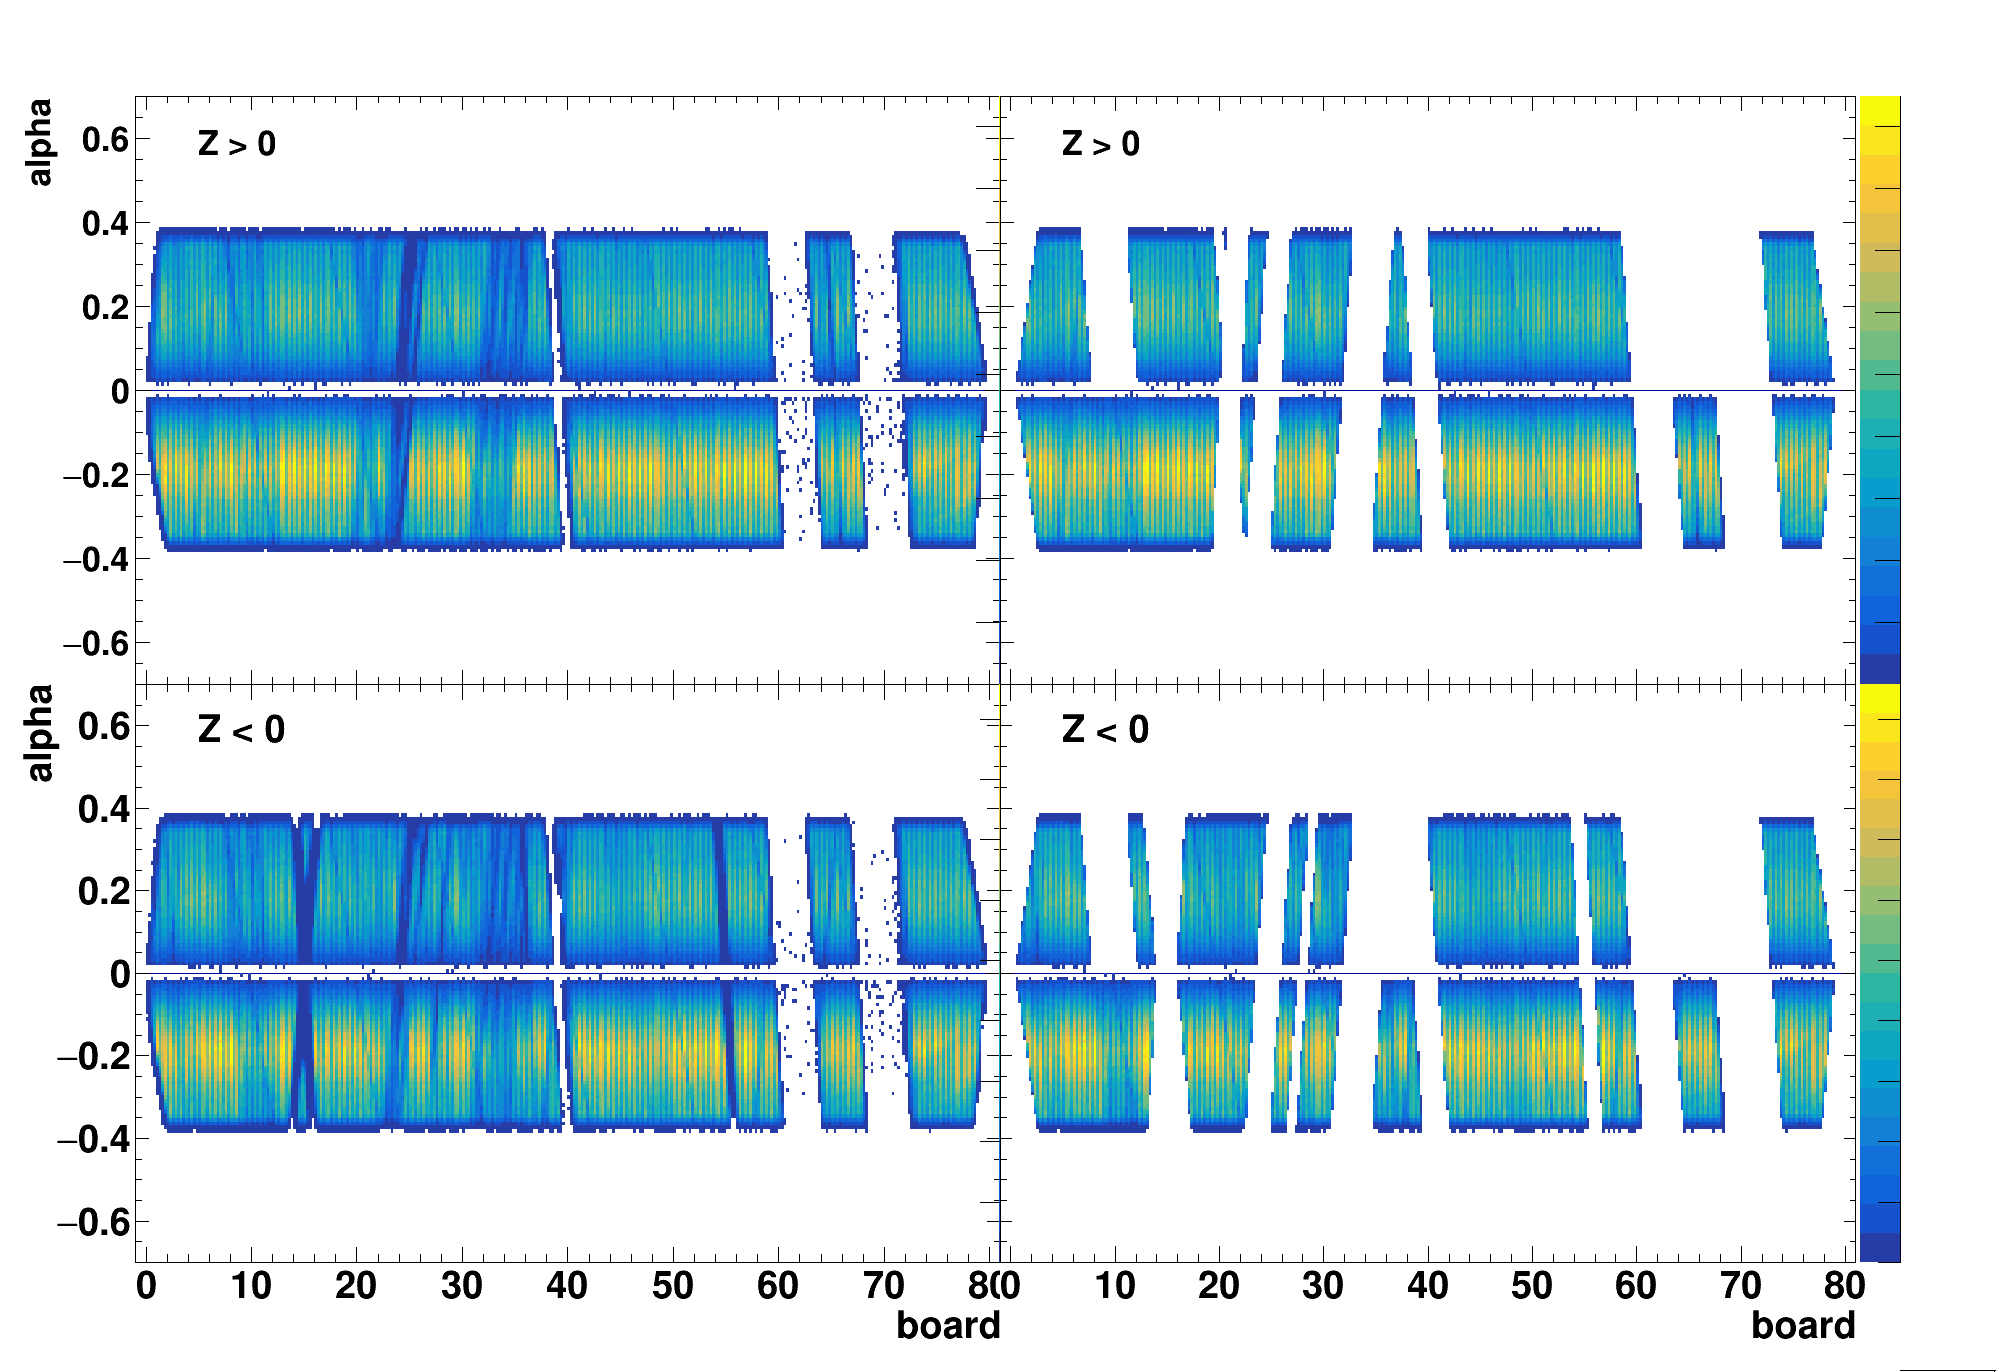
\includegraphics [width=0.8\linewidth]{Methodology/DC_DM_pAl.png}
	\caption{Гистограмма загрузки дрейфовых камер в 2015 году} 
	\label{img:Met_DMRun15}
\end{figure}


\subsection{Измерение первичного выхода заряженных адронов} \label{sect3_PID}
Заряженные адроны регистрируются непосредственно с помощью времяпролетной и дрейфовых камер эксперимента PHENIX. Квадрат массы частиц, зарегистрированных во времяпролетной и дрейфовой камерах, может быть определен в соответствии с выражением \ref{eq:TOFm2}:
\begin{equation}
m^2 = \frac{p^2}{c^2} \left( \frac{t^2 c^2}{L^2} - 1\right),
\label{eq:TOFm2}
\end{equation}
где $p$ -- импульс частицы, измеренный с помощью дрейфовой камеры; 

$L$ -- длина, пройденная частицей от вершины взаимодействия до места регистрации во времяпролетной камере; 

$t$ -- время, прошедшее с момента столкновения ионов до момента регистрации образовавшейся частицы во времяпролетной камере; 

$c$ -- скорость света.
На Рисунке \ref{img:TOF_PID} а) представлено распределение произведения квадрата массы и заряда регистрируемых адронов в зависимости от поперечного импульса, полученное в соответствии с выражением \ref{eq:TOFm2}.


\begin{table}[]
	\caption{\pt-интервалы измерений заряженных адронов в \pal, \heau, Cu+Au и U+U системах столкновений.}
	\label{table:pt_ranges}
	
	\begin{tabularx}{\linewidth}
		{
			| >{\centering\arraybackslash}X
			| >{\centering\arraybackslash}X
			| >{\centering\arraybackslash}X
			| >{\centering\arraybackslash}X
			| >{\centering\arraybackslash}X | }
		\hline
	\pt (ГэВ/$c$) &  \pal & \heau  & Cu+Au & U+U  \\ \hline
	\pip  & 0,5 - 2,0  &  0,5 - 3,0  &  0,5 - 3,0  & 0,5 - 3,5  \\
	\pim  & 0,5 - 2,0  &  0,5 - 2,0  &  0,5 - 3,0  & 0,5 - 3,0  \\
	\Kp   & 0,5 - 1,8  &  0,5 - 2,0  &  0,5 - 2,0  & 0,5 - 2,0  \\
	\Km   & 0,5 - 1,8  &  0,5 - 2,0  &  0,5 - 2,0  & 0,5 - 2,0  \\
	\prot &  &  0,5 - 4,0  &  0,5 - 4,0  &    0,5 - 4,0     \\
	\aprot & 0,5 - 2,5  &  0,5 - 4,0  &  0,5 - 4,0  &  0,5 - 4,0 \\ \hline
		
	\end{tabularx}
\end{table}

% Сигналы, соответствующие протонам, каонам и пионам, на данном распределении хорошо различимы.

Для идентификации типа частиц, сигналы, зарегистрированные в TOF, аппроксимируются функциями Гаусса со среднеквадратичными отклонениями ($\sigma_{TOF}$) и математическими ожиданиями ($m_{TOF}^2$) в каждом интервале $\Delta p_T = 0,5$ ГэВ/$c$ диапазона \pt \ идентификации адронов. Диапазоны идентификации адронов по \pt \ приведены в табл.~\ref{table:pt_ranges}.  Пример аппроксимации в диапазоне поперечных импульсов 1,0 -- 1,1 ГэВ/с представлен на Рисунке \ref{img:TOF_PID} б). Далее для каждого типа адрона $h$ ($h = \pi^{\pm}$, $K^{\pm}$, $p$, $\bar{p}$) полученные дискретные зависимости $\sigma_{TOF_{h}}(p_T)$ и $m_{TOF_{h}}^2(p_T)$ параметризуются уравнением ~\ref{eq:TOFgaus_approx}. 
\begin{equation}
	m_{TOF_{h}}^2(p_T),\sigma_{TOF_{h}}(p_T) = p_0 +\frac{p_1}{p_T} + \frac{p_2}{p_T^2} + p_3 \cdot e^{\sqrt{p_T}} +p_4 \cdot \sqrt{p_T},
	\label{eq:TOFgaus_approx}
\end{equation}

Значения $\sigma_{TOF_{h}}$ и $m_{TOF_{h}}^2$, вычисленные по формуле \ref{eq:TOFgaus_approx}, используются для идентификации частиц. Частица с зарегистрированным квадратом массы $m_{TOF}^2$ идентифицируется как адрон $h$ в том случае, если  $m_{TOF}^2$ удовлетворяет неравенствам 
$$ m_{TOF_{h}}^2 -2\sigma_{TOF_{h}} < m_{TOF}^2 < m_{TOF_{h}}^2 +2\sigma_{TOF_{h}}. $$
При значениях поперечных импульсов \pt \ $\sim$ 2 -- 3 ГэВ/$с$ происходит наложение сигналов заряженных адронов. В связи с этим было введено дополнительное условие, обеспечивающее непопадание массы частицы в диапазон $\pm 2\sigma_{TOF_{h}}$ соседних сигналов частиц.
Условия идентификации заряженных адронов приведены в Таблице \ref{table:m2cuts}.


\begin{comment}
Диапазон поперечных импульсов разбивается на промежутки шириной 0,1 ГэВ/с, на каждом из которых сигналы заряженных адронов аппроксимируются функцией Гаусса. Пример такой аппроксимации в диапазоне поперечных импульсов 1,0-1,1 ГэВ/с представлен на рис. \ref{img:TOF_PID}. 
Далее зависимости от поперечного импульса полученных среднеквадратичных отклонений ($\Tilde{\sigma}_h$) и математических ожиданий ($\Tilde{m}^2_h$) функций Гаусса для адронов h (h=\pipm,\Kpm,\prot, \aprot ) аппроксимировались функцией  \ref{eq:TOFgaus_approx}.

\begin{equation}
	\label{eq:TOFgaus_approx}
	f(p_T) = P_0 +P_1/p_T + P_2/p_T^2 + P_3 \cdot exp(\sqrt{p_T}) +P_4 \cdot \sqrt{p_T} 
\end{equation}
где $P_i, i \in [1,4]$ - параметры аппроксимации.

Значения $\sigma_h$ и $m_h$, вычисленные по формуле \ref{eq:TOFgaus_approx}, использовались для идентификации частиц. Частица, с зарегистрированным квадратом массы $m^2$, идентифицируется как адрон h в том случае, если  $m^2$ удовлетворяет неравенствам $$ m^2_h -2\sigma_h < m^2 < m^2_h +2\sigma_h. $$
При значениях поперечных импульсов \pt~2-3 ГэВ/с происходит наложение сигналов заряженных адронов. В связи с этим было введено дополнительное условие, обеспечивающее непопадание массы частицы в диапазон $\pm 2\sigma_h$ соседних сигналов частиц.
Условия идентификации заряженных адронов приведены в таблице \ref{table:m2cuts}.
\end{comment}

\begin{table}[]
	\caption{Условия идентификации частиц}
	\label{table:m2cuts}
	\begin{center}
		\begin{tabular}{|c|c|}
			\hline
			\multirow{2}{*}{\pipm} & $|m^2_{TOF} - m^2_{TOF_{\pi}}|<2\sigma_{TOF_{\pi}}$ \\ 
			& $m^2_{TOF} < m^2_{TOF_{K}}-2\sigma_{TOF_{K}}$ \\ \hline
			\multirow{3}{*}{\Kpm}  & $|m^2 - m^2_{TOF_{K}}|<2\sigma_{TOF_{K}}$  \\ 
			& $m^2_{TOF} > m^2_{TOF_{\pi}}+2\sigma_{TOF_{\pi}}$\\  
			& $m^2_{TOF} < m^2_{TOF_{p}}+2\sigma_{TOF_{p}}$ \\ \hline
			\multirow{2}{*}{\prot, \aprot} & $|m^2_{TOF} - m^2_{TOF_{p}}|<2\sigma_{TOF_{p}}$ \\ 
			& $m^2_{TOF} > m^2_{TOF_{K}}+2\sigma_{TOF_{K}}$ \\ \hline
		\end{tabular}
	\end{center}
\end{table}



\begin{figure}[ht] 
	\centerfloat
	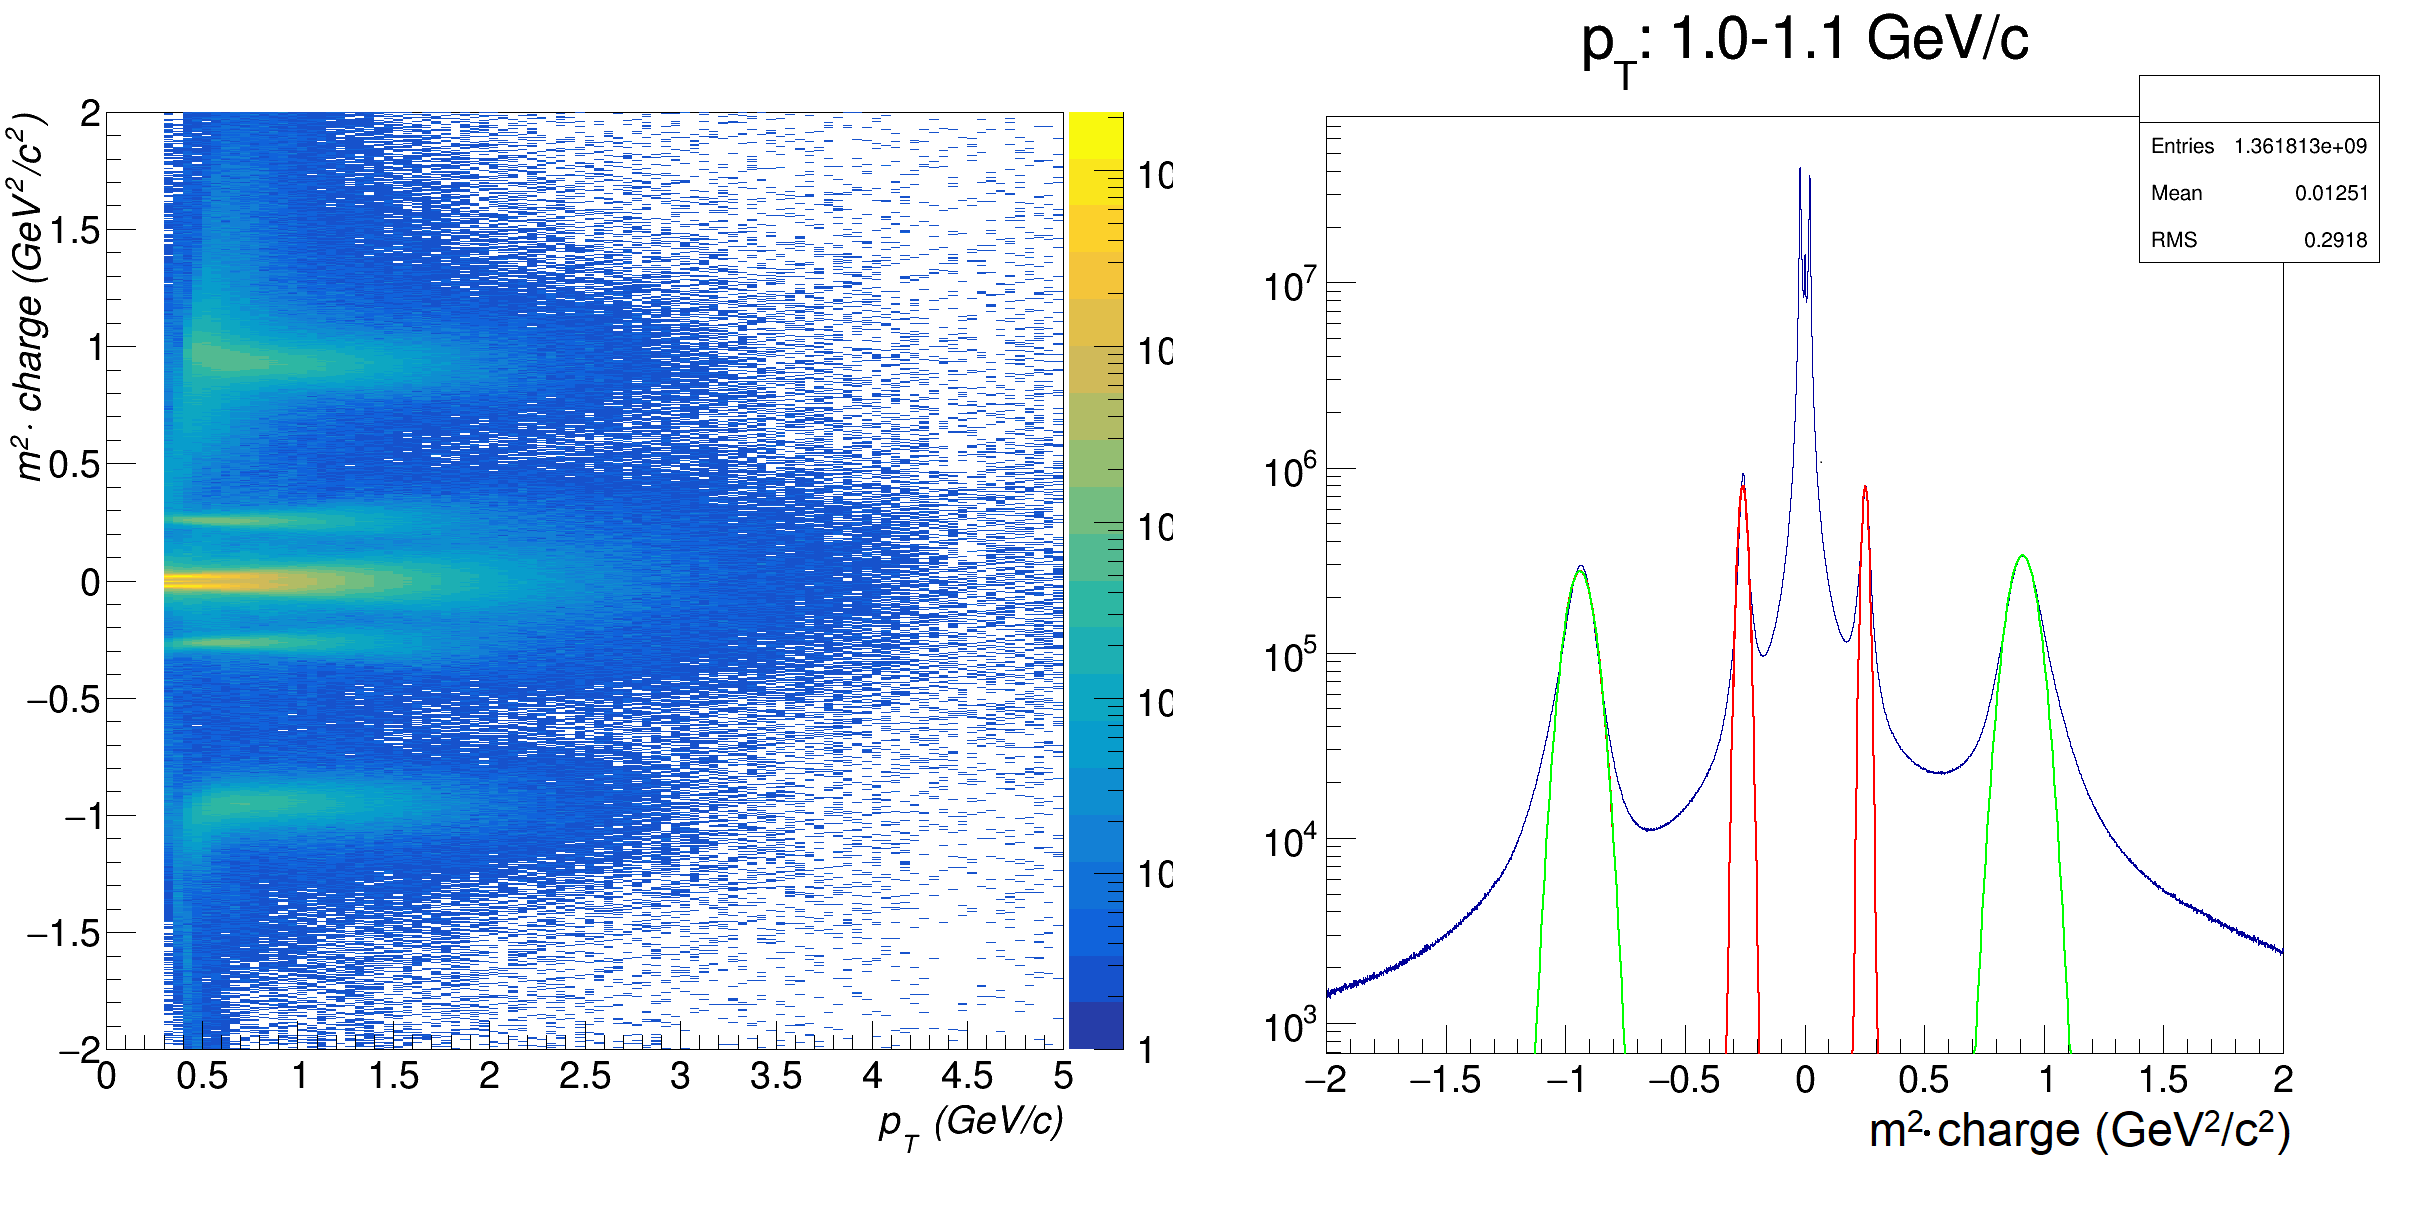
\includegraphics [width = 0.9\linewidth] {Methodology/TOF2.png}
	\caption{а) Двухмерное распределение произведения квадрата массы на заряд регистрируемых адронов в зависимости от поперечного импульса б) Пример аппроксимации сигналов от заряженных адронов функцией Гаусса в диапазоне поперечных импульсов 1,0 -- 1,1 ГэВ/с} 
	\label{img:TOF_PID}  
\end{figure}

\section{Оценка коррекций измерения первичного выхода заряженных адронов}

\subsection{Оценка эффективности регистрации} \label{sect3:EffRec}

%To correct for geometrical acceptance, analysis cuts, particle interactions with detector materials, and in-flight decays (for pions and kaons), we use single particle Monte Carlo (MC) simulations. For these simulations, single particles are generated using a random generator, with flat distributions in rapidity, azimuth, and \pT. The random particles are then run through a geant simulation of PHENIX to determine the interactions of the single particles with the detector subsystems and support structures. Next, all the detector response information is fed through the usual PHENIX reconstruction software to produce simulated tracks. Finally, these simulated tracks are analyzed in the exact same way as tracks from the real data in order to determine the corrections. The total correction factor, FC(\pT), is given by the following relation:

%\begin{equation}
%  \label{eq:CorrFactor}
%    FC(p_T) = %\frac{dN_{output}/dp_T}{dN_{input}/dp_T} = %\epsilon_{acceptance}\epsilon_{efficiency}\epsilon{cuts}
%\end{equation}
%To correct for the detector occupancy effect, which is most significant in the TOFW, we run embedding simulations, where a track from single particle MC simulations is embedded into a real event, and the occupancy correction is determined from the relative efficiencies of reconstructing the single track in isolation and in the event. This correction is the largest in the most central Au+Au collisions where the multiplicity is the highest and therefore the occupancy effect is the strongest. In the most peripheral Au+Au collisions the multiplicity is low enough that there is essentially no effect. The same is true in d+Au collisions, where no correction is applied.

Для того чтобы оценить количество адронов, родившихся в вершине ядро-ядерных взаимодействий, измеренные значения первичного выхода адронов должны быть скорректированы на эффективность регистрации ($\epsilon_{reg}$) адронов, учитывающей ограниченный аксептанс времяпролетной камеры, детекторные эффекты (различные шумы, разрешение и калибровка, нелинейность, эффективность триггеров реального времени и т.д.) и используемые при отборе данных ограничения.

Оценка эффективности регистрации частиц была проведена с помощью метода Монте-Карло.
Частицы с заданными массами покоя, координатами вершины рождения, энергией генерируются с помощью генератора  случайных чисел с плоскими распределениями по быстроте, азимуту и поперечному импульсу \pt. Затем сгенерированные частицы поступают в качестве входных данных в программный пакет PISA для определения взаимодействия отдельных частиц с подсистемами детектора PHENIX. 

PISA (PHENIX Integrated Simulation Application) является программой моделирования ядро-ядерных столкновений методом Монте-Карло, разработанного для детектора PHENIX на основе GEANT3.
Программа PISA учитывает геометрию, пространственное расположение и материал изготовления детекторных подсистем спектрометра PHENIX, их пространственные, импульсные и энергетические разрешения, а также конфигурация магнитного поля, полностью соответствующие структуре реальной установки в данном цикле ядро-ядерных столкновений.

%Информация, полученная в результате работы программы GEANT4 обрабатывается с помощью стандартного программного обеспечения эксперимента  PHENIX для реконструкции треков.Наконец, ...
Для обработки данных, полученных в результате моделирования, применяются те же критерии отбора событий и идентификации частиц, что и для экспериментальных данных (см. Раздел \ref{sect3_cuts}).

Функция эффективности регистрации вычисляется согласно следующему соотношению:
$$\epsilon_{reg} = \frac{N_{reg}(p_T)}{N_{tot}(p_T)},$$
где $N_{reg}$ -- количество адронов, зарегистрированных в Монте-Карло модели,

$N_{tot}$ -- общее количество адронов, разыгранное в Монте-Карло модели.
Эффективность регистрации, рассчитанная согласно приведенному соотношению, учитывает геометрические параметры детектора.

Полученные значения эффективности регистрации идентифицируемых заряженных адронов представлены на Рисунках \ref{img:eff_pAl}-\ref{img:eff_UU}. Малые значения эффективности регистрации ($\sim1 \%$) объясняются небольшим размером TOF (2450мм $\times$ 1924мм). Различия в значениях $\epsilon_{rec}$, полученными в различных системах столкновений, обусловлены различной конфигурацией и износом детекторной системы в различные годы набора данных.
%Входными данными для проекта PISA являются выборки частиц со случайно разыгранными величинами характеристик: координатами вершины рождения, массой покоя, каналом распада, энергией и проекциями импульса, моделирующие спектр частиц, рожденных в процессе ядро-ядерных столкновений. Розыгрыш этих характеристик формируется в соответствии с плоскими распределениями по вершине вдоль оси $z$ поперечному импульсу, псевдобыстроте и азимутальному углу смоделированных частиц. 
В Таблице \ref{tab:Met_sim} приведены числа событий и границы изменения величин вершины, поперечного импульса, псевдобыстроты и азимутального угла в смоделированных выборках для исследуемых адронов.

\begin{table}[h]
	\centering
	\caption{Параметры моделирования}
	\begin{tabular}{|c|c|c|c|c|c|c|}
		\hline
		Частица &
		\begin{tabular}[c]{@{}l@{}}Количество\\ событий\end{tabular} & 
		$\Delta$ y& 
		\begin{tabular}[c]{@{}l@{}}$\phi$\\ рад\end{tabular}& \begin{tabular}[c]{@{}l@{}}$p_T^{max}$\\ ГэВ/с\end{tabular} & \begin{tabular}[c]{@{}l@{}}$p_T^{min}$\\ ГэВ/с\end{tabular} & \begin{tabular}[c]{@{}l@{}}Вершина\\см\end{tabular} \\ 
		\hline \pip & $10 \cdot 10^6$ & -0,5 - 0,5 & $\pi/2 - 3\pi/2$ & 0,0 & 3,5 & -30 - 30 \\
		\hline \pim & $10 \cdot 10^6$ & -0,5 - 0,5 & $\pi/2 - 3\pi/2$ & 0,0 & 3,5 & -30 - 30 \\
		\hline \Kp & $10 \cdot 10^6$ & -0,5 - 0,5 & $\pi/2 - 3\pi/2$ & 0,0 & 2 & -30 - 30 \\
		\hline \Km & $10 \cdot 10^6$ & -0,5 - 0,5 & $\pi/2 - 3\pi/2$ & 0,0 & 2 & -30 - 30 \\
		\hline \prot & $10 \cdot 10^6$ & -0,5 - 0,5 & $\pi/2 - 3\pi/2$ & 0,0 & 5 & -30 - 30 \\
		\hline \aprot & $10 \cdot 10^6$ & -0,5 - 0,5 & $\pi/2 - 3\pi/2$ & 0,0 & 5 & -30 - 30 \\
		\hline
	\end{tabular}
	\label{tab:Met_sim}
\end{table}

Перед расчетом эффективности регистрации была выполнена проверка соответствия данных моделирования и экспериментальных данных путем сравнения распределений треков в данных выборках. Гистограмма распределения треков в зависимости от номера <<платы>> ДК, полученная путем моделирования, была нормирована в соответствии с экспериментальными данными. Результаты сравнения распределений треков в ДК представлены на Рисунке \ref{img:DC_compar}. Результаты моделирования соответствуют результатам, полученным в эксперименте.

Аналогичная проверка была выполнена для восточного крыла времяпролетной камеры (TOFE). Гистограммы распределения треков на плоскость $z-y$ детектора TOFE, полученные с использованием экспериментальных данных и данных моделирования представлены на Рисунках \ref{img:TOFproj_pAl}-\ref{img:TOFproj_CuAu}. Проекции двухмерных гистограмм \ref{img:TOFproj_pAl}-\ref{img:TOFproj_CuAu} на оси $y$ и $z$ представлены на верхней и нижней панелях соответственно на Рисунках \ref{img:TOFproj_pAl}-\ref{img:TOFproj_CuAu}.  Результаты моделирования также соответствуют результатам, полученным в эксперименте.

\begin{figure}[] 
	\centerfloat
	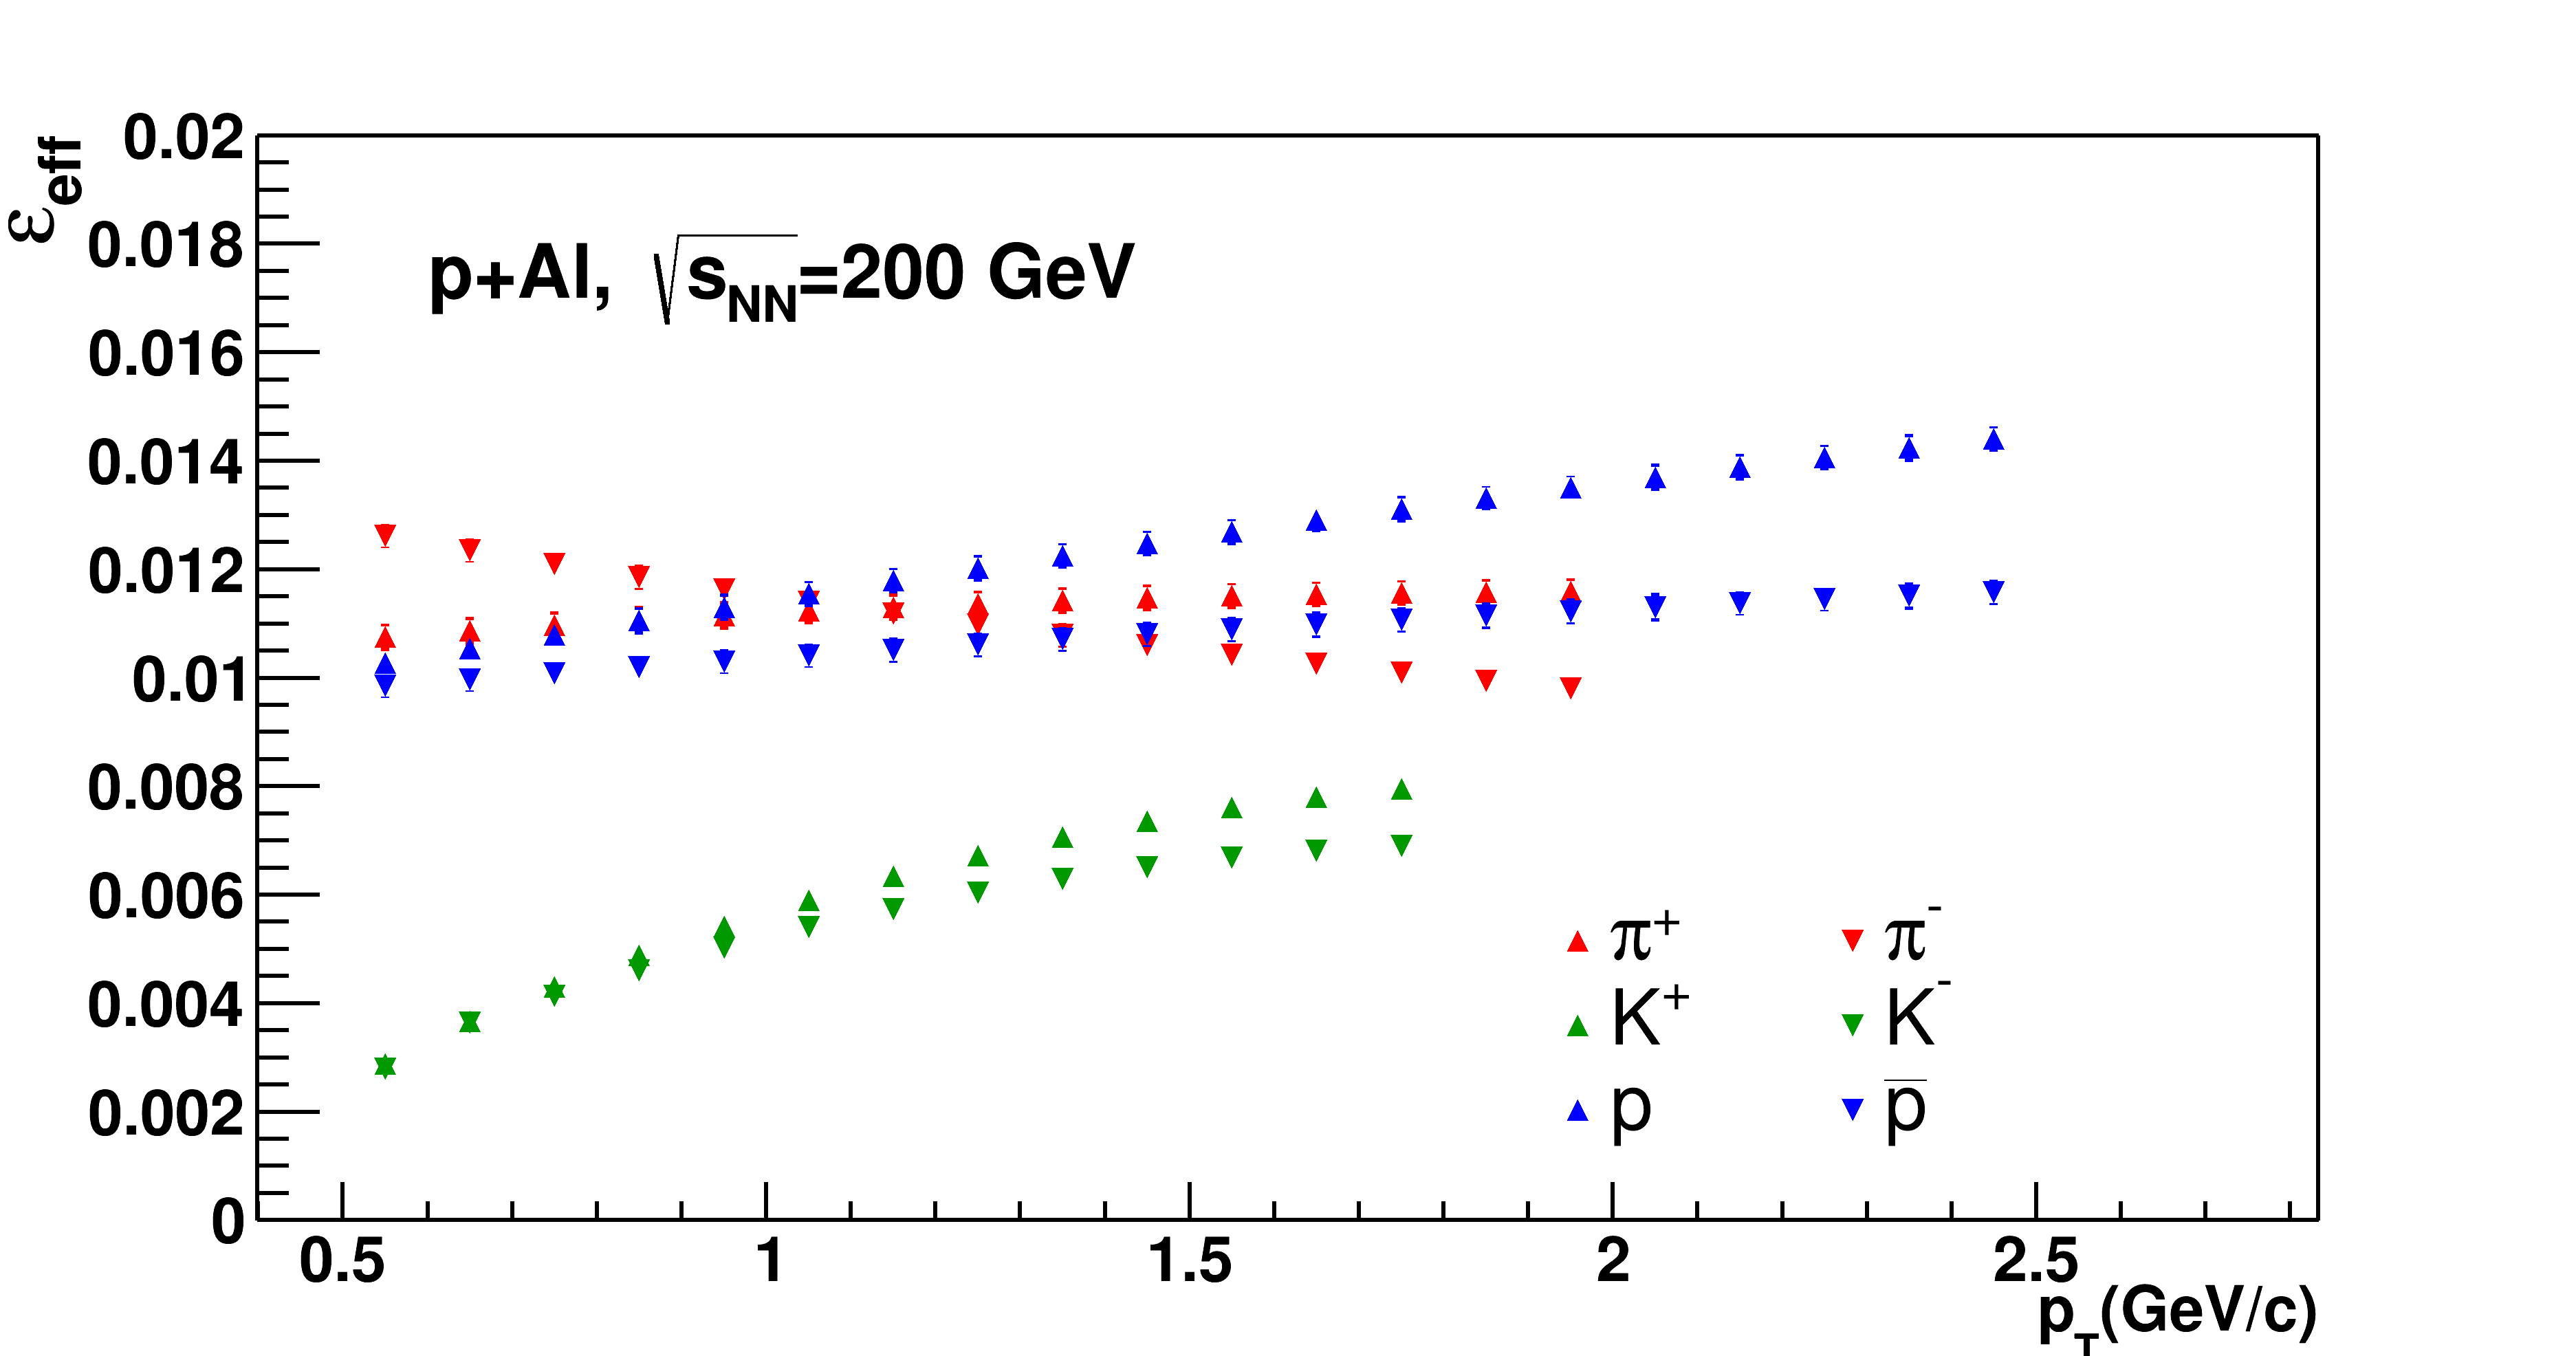
\includegraphics [width=0.9\linewidth]{Methodology/eff_hadron_pAl.png}
	\caption{Эффективность регистрации заряженных адронов в столкновениях \pal.} 
	\label{img:eff_pAl}
\end{figure}

\begin{figure}[] 
	\centerfloat
	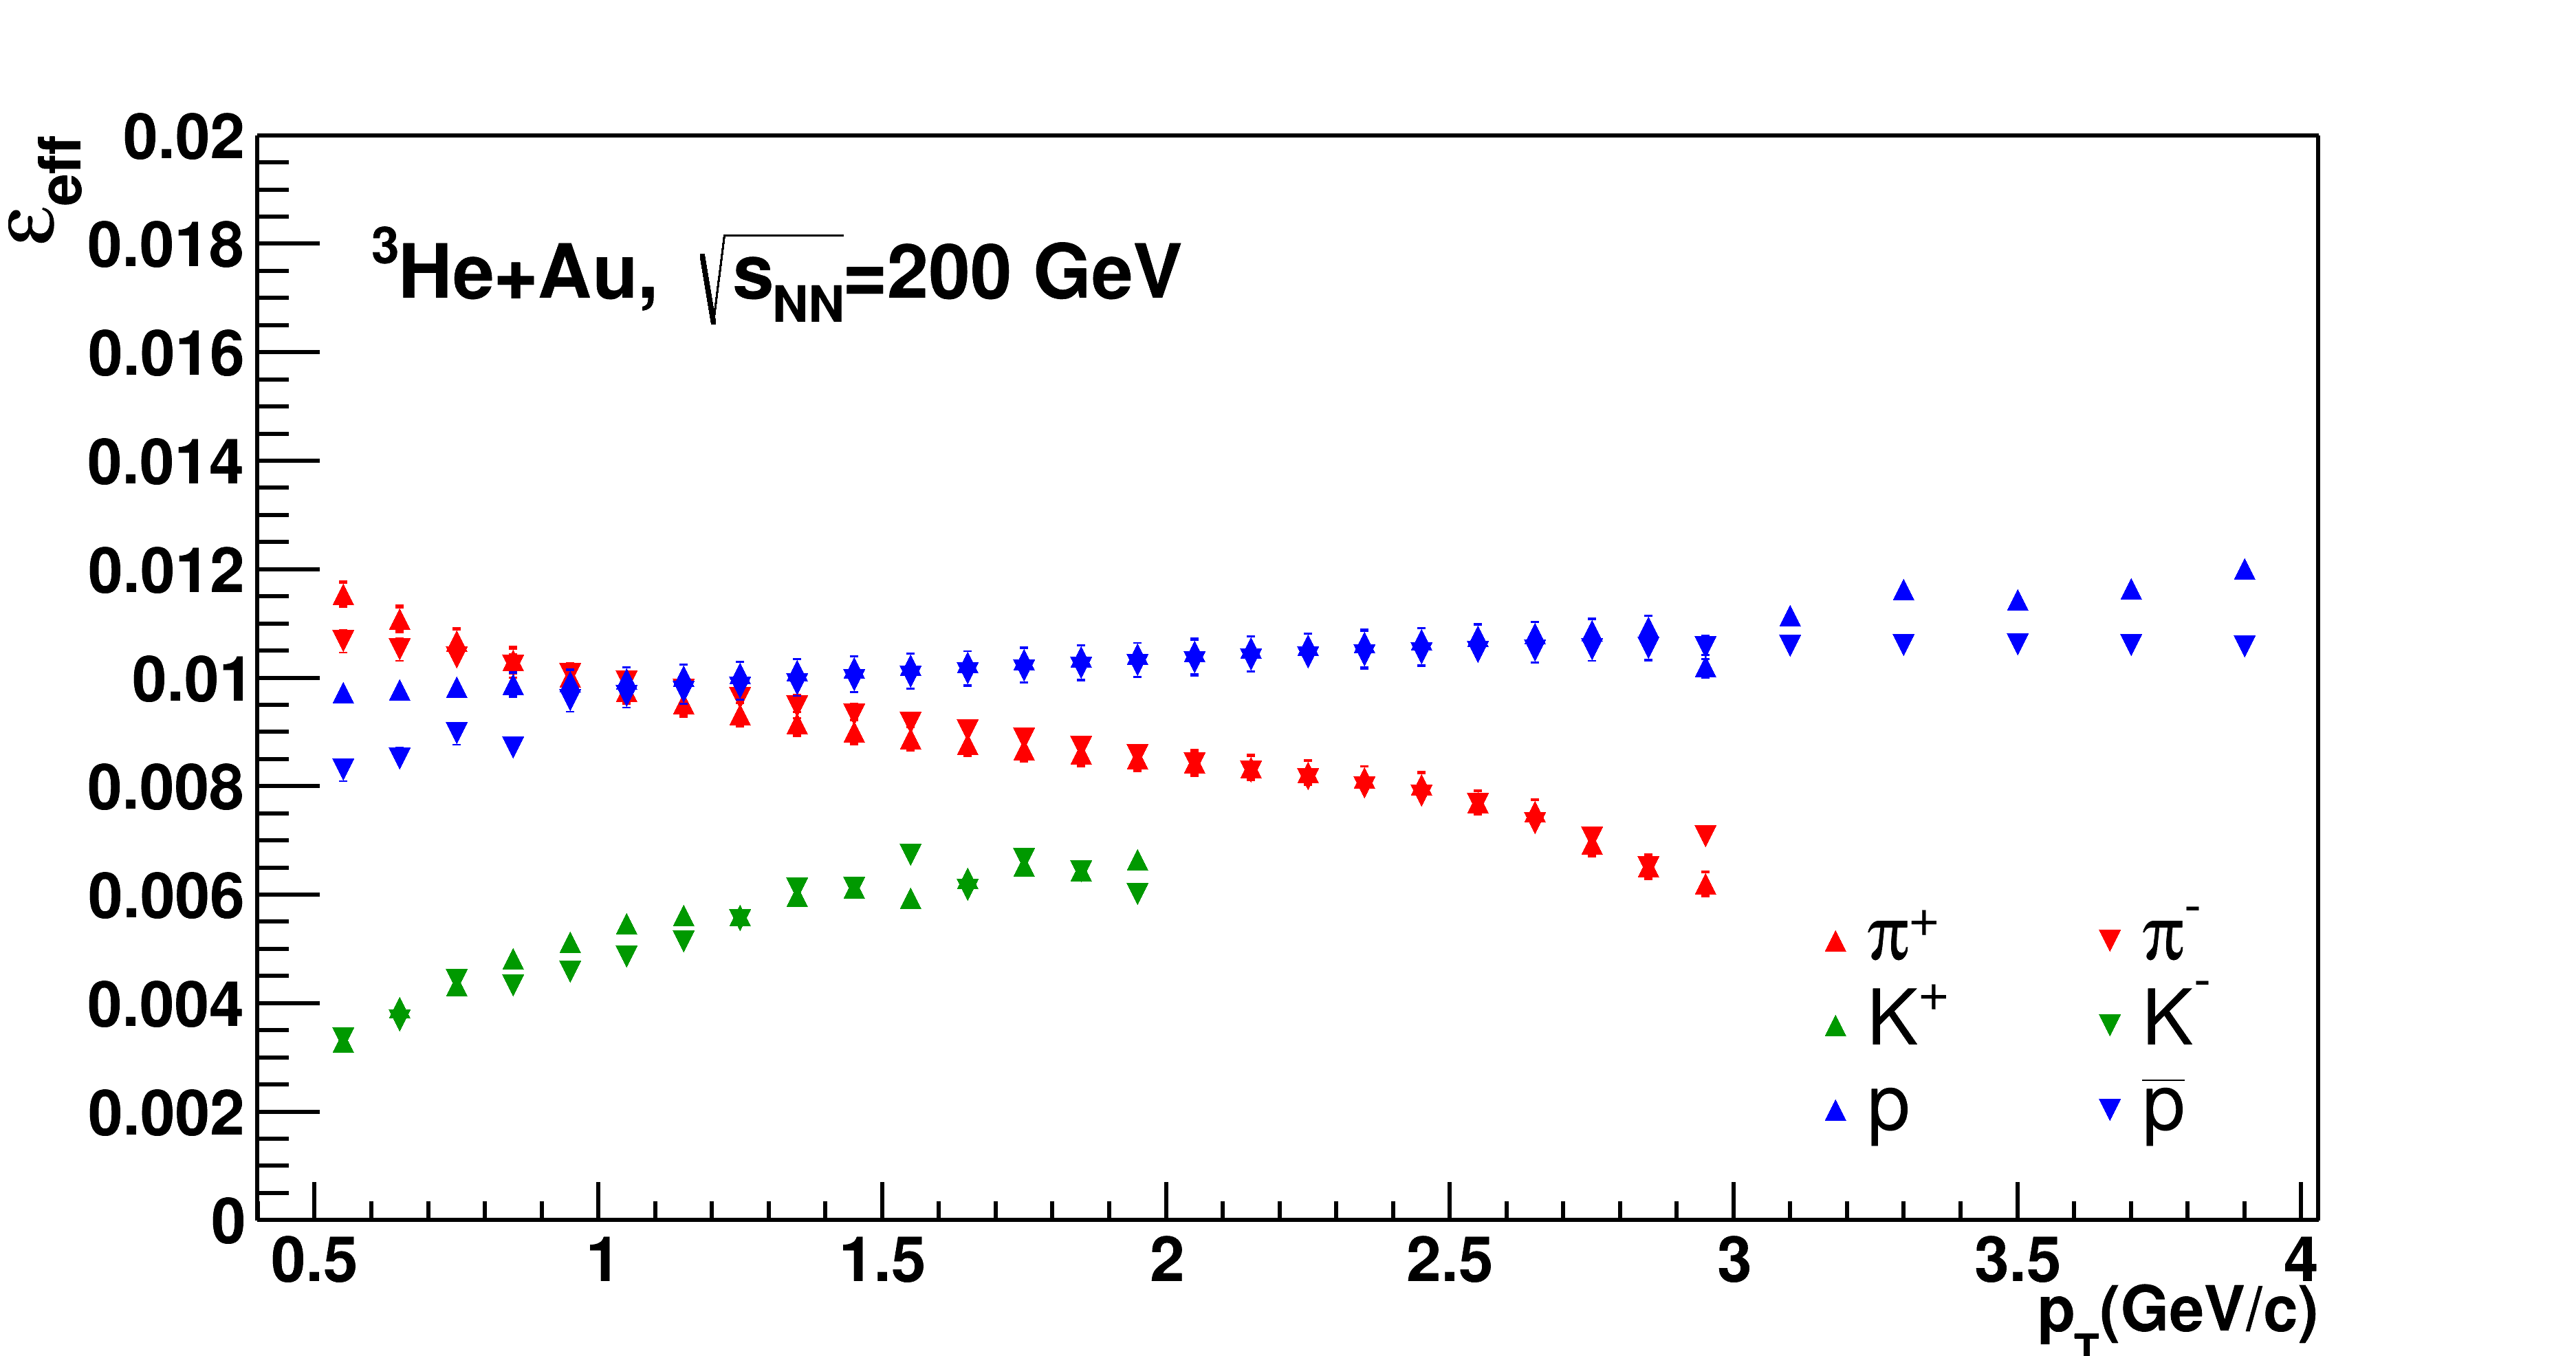
\includegraphics [width=0.9\linewidth]{Methodology/eff_hadron_HeAu.png}
	\caption{Эффективность регистрации заряженных адронов в столкновениях \heau.} 
	\label{img:eff_HeAu}
\end{figure}

\begin{figure}[] 
	\centerfloat
	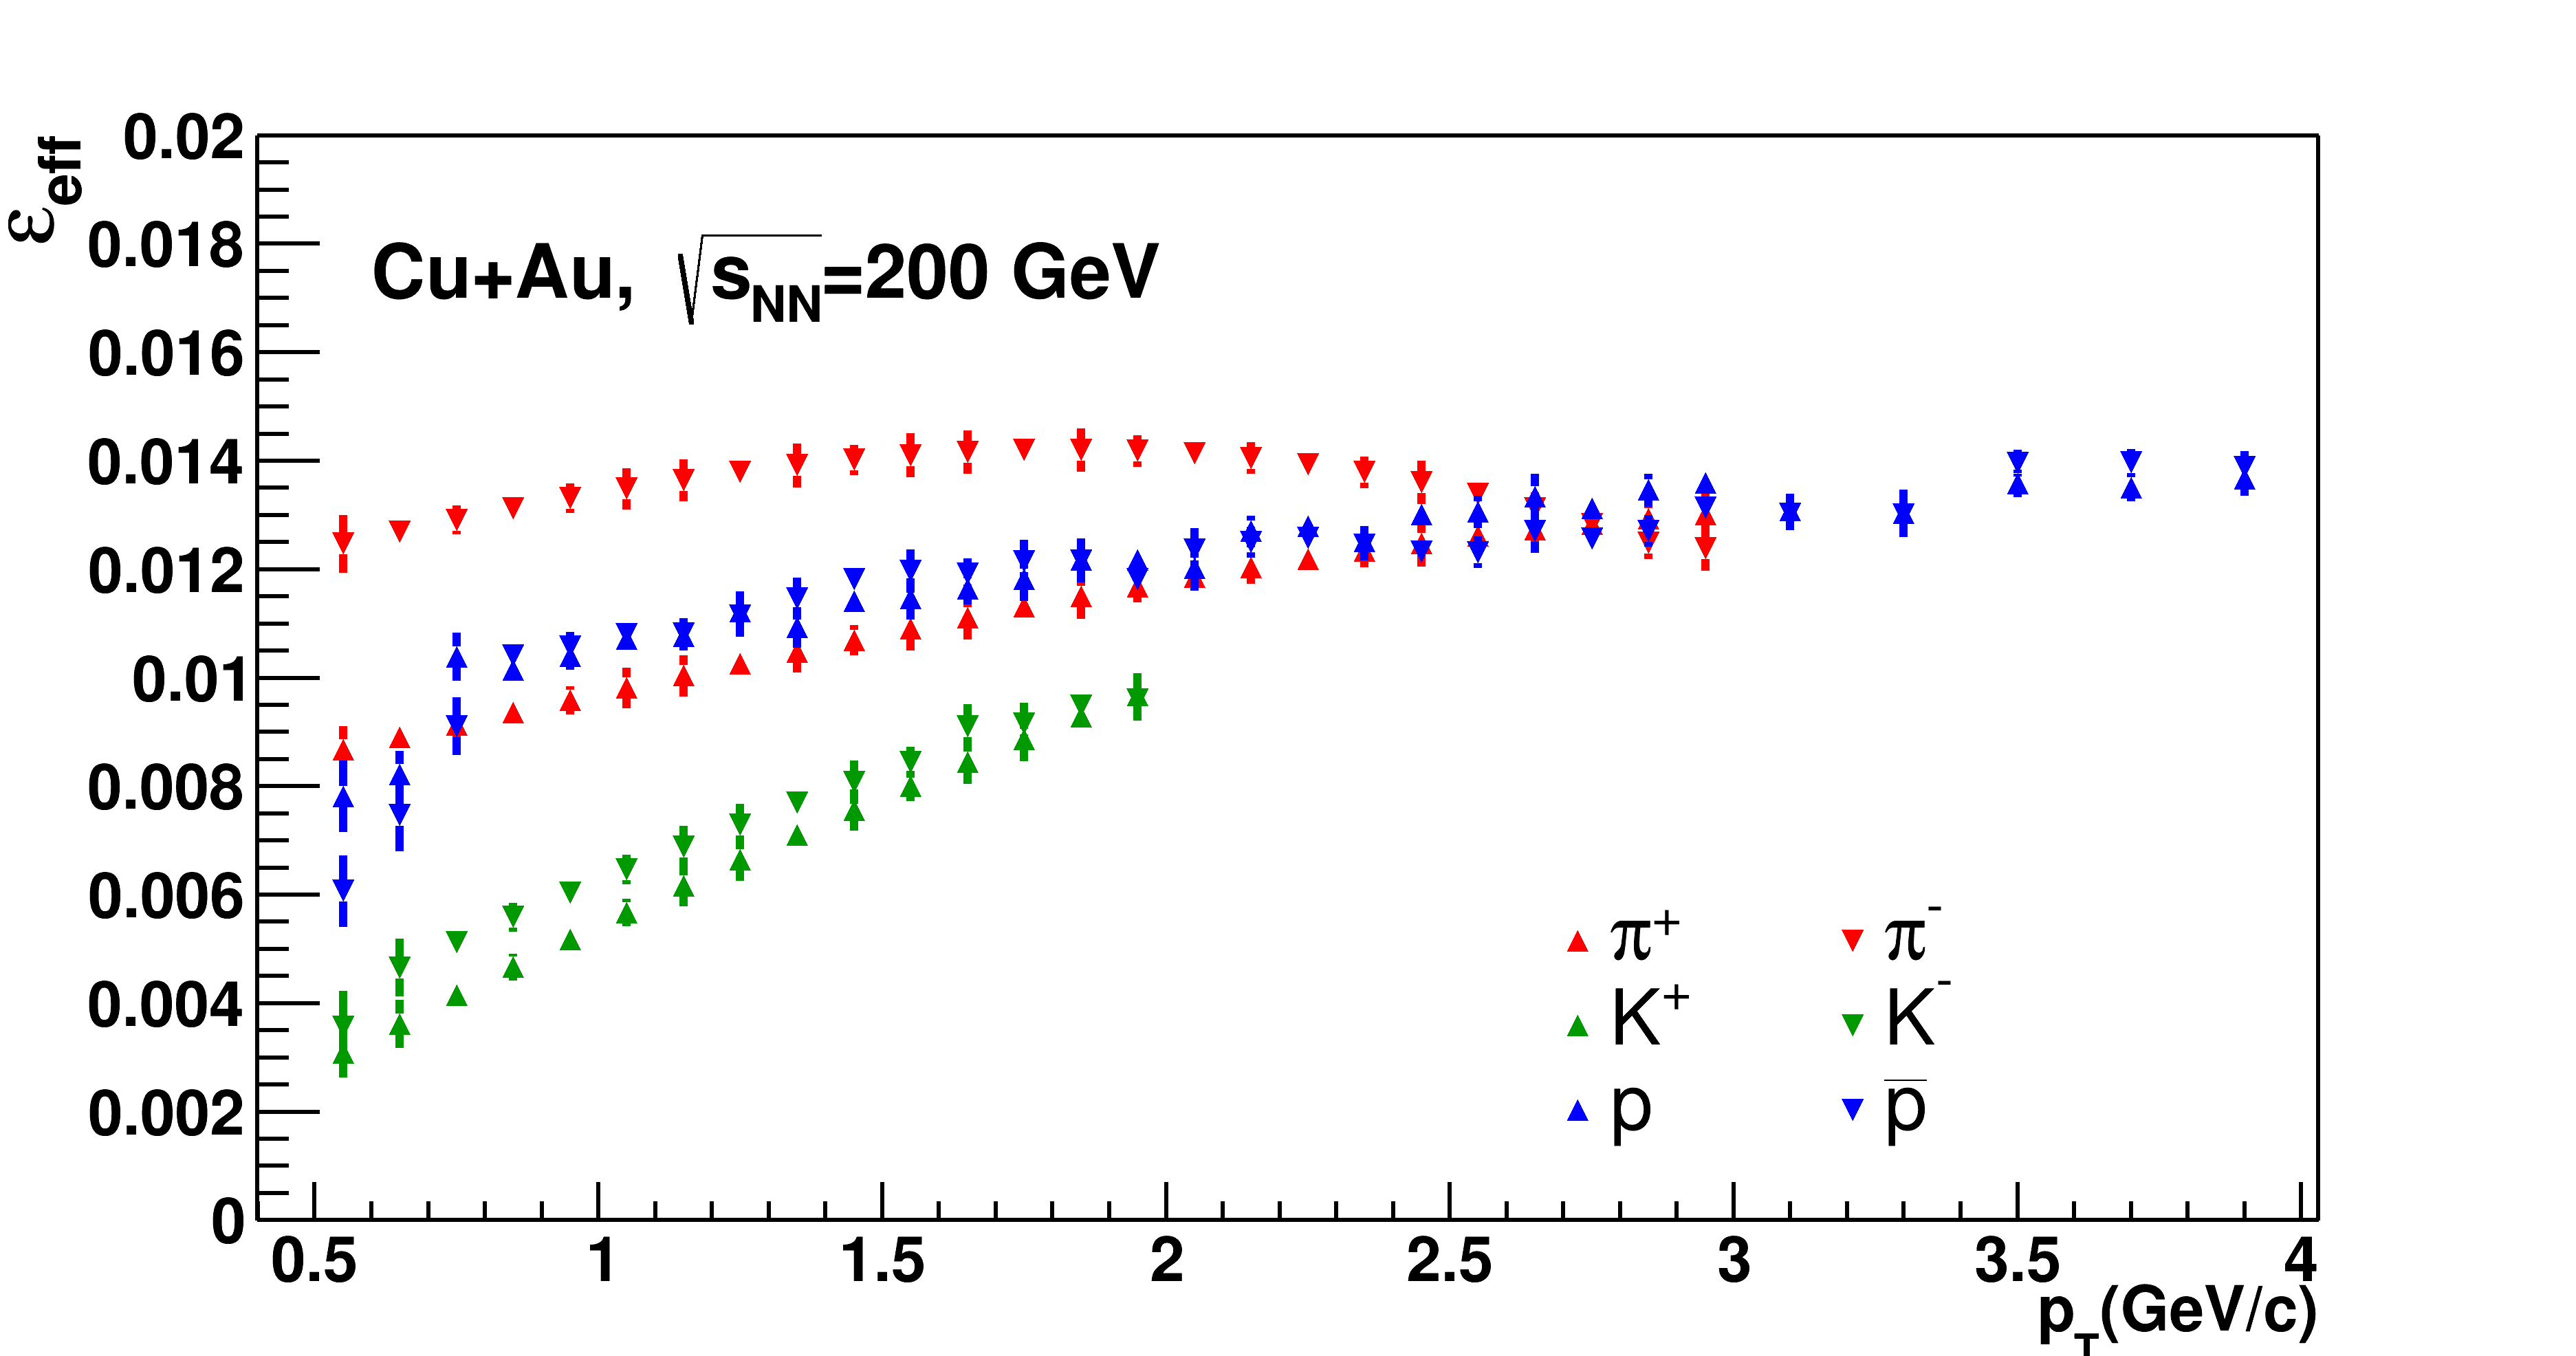
\includegraphics [width=0.9\linewidth]{Methodology/eff_hadron_CuAu.png}
	\caption{Эффективность регистрации заряженных адронов в столкновениях Cu+Au.} 
	\label{img:eff_CuAu}
\end{figure}

\begin{figure}[] 
	\centerfloat
	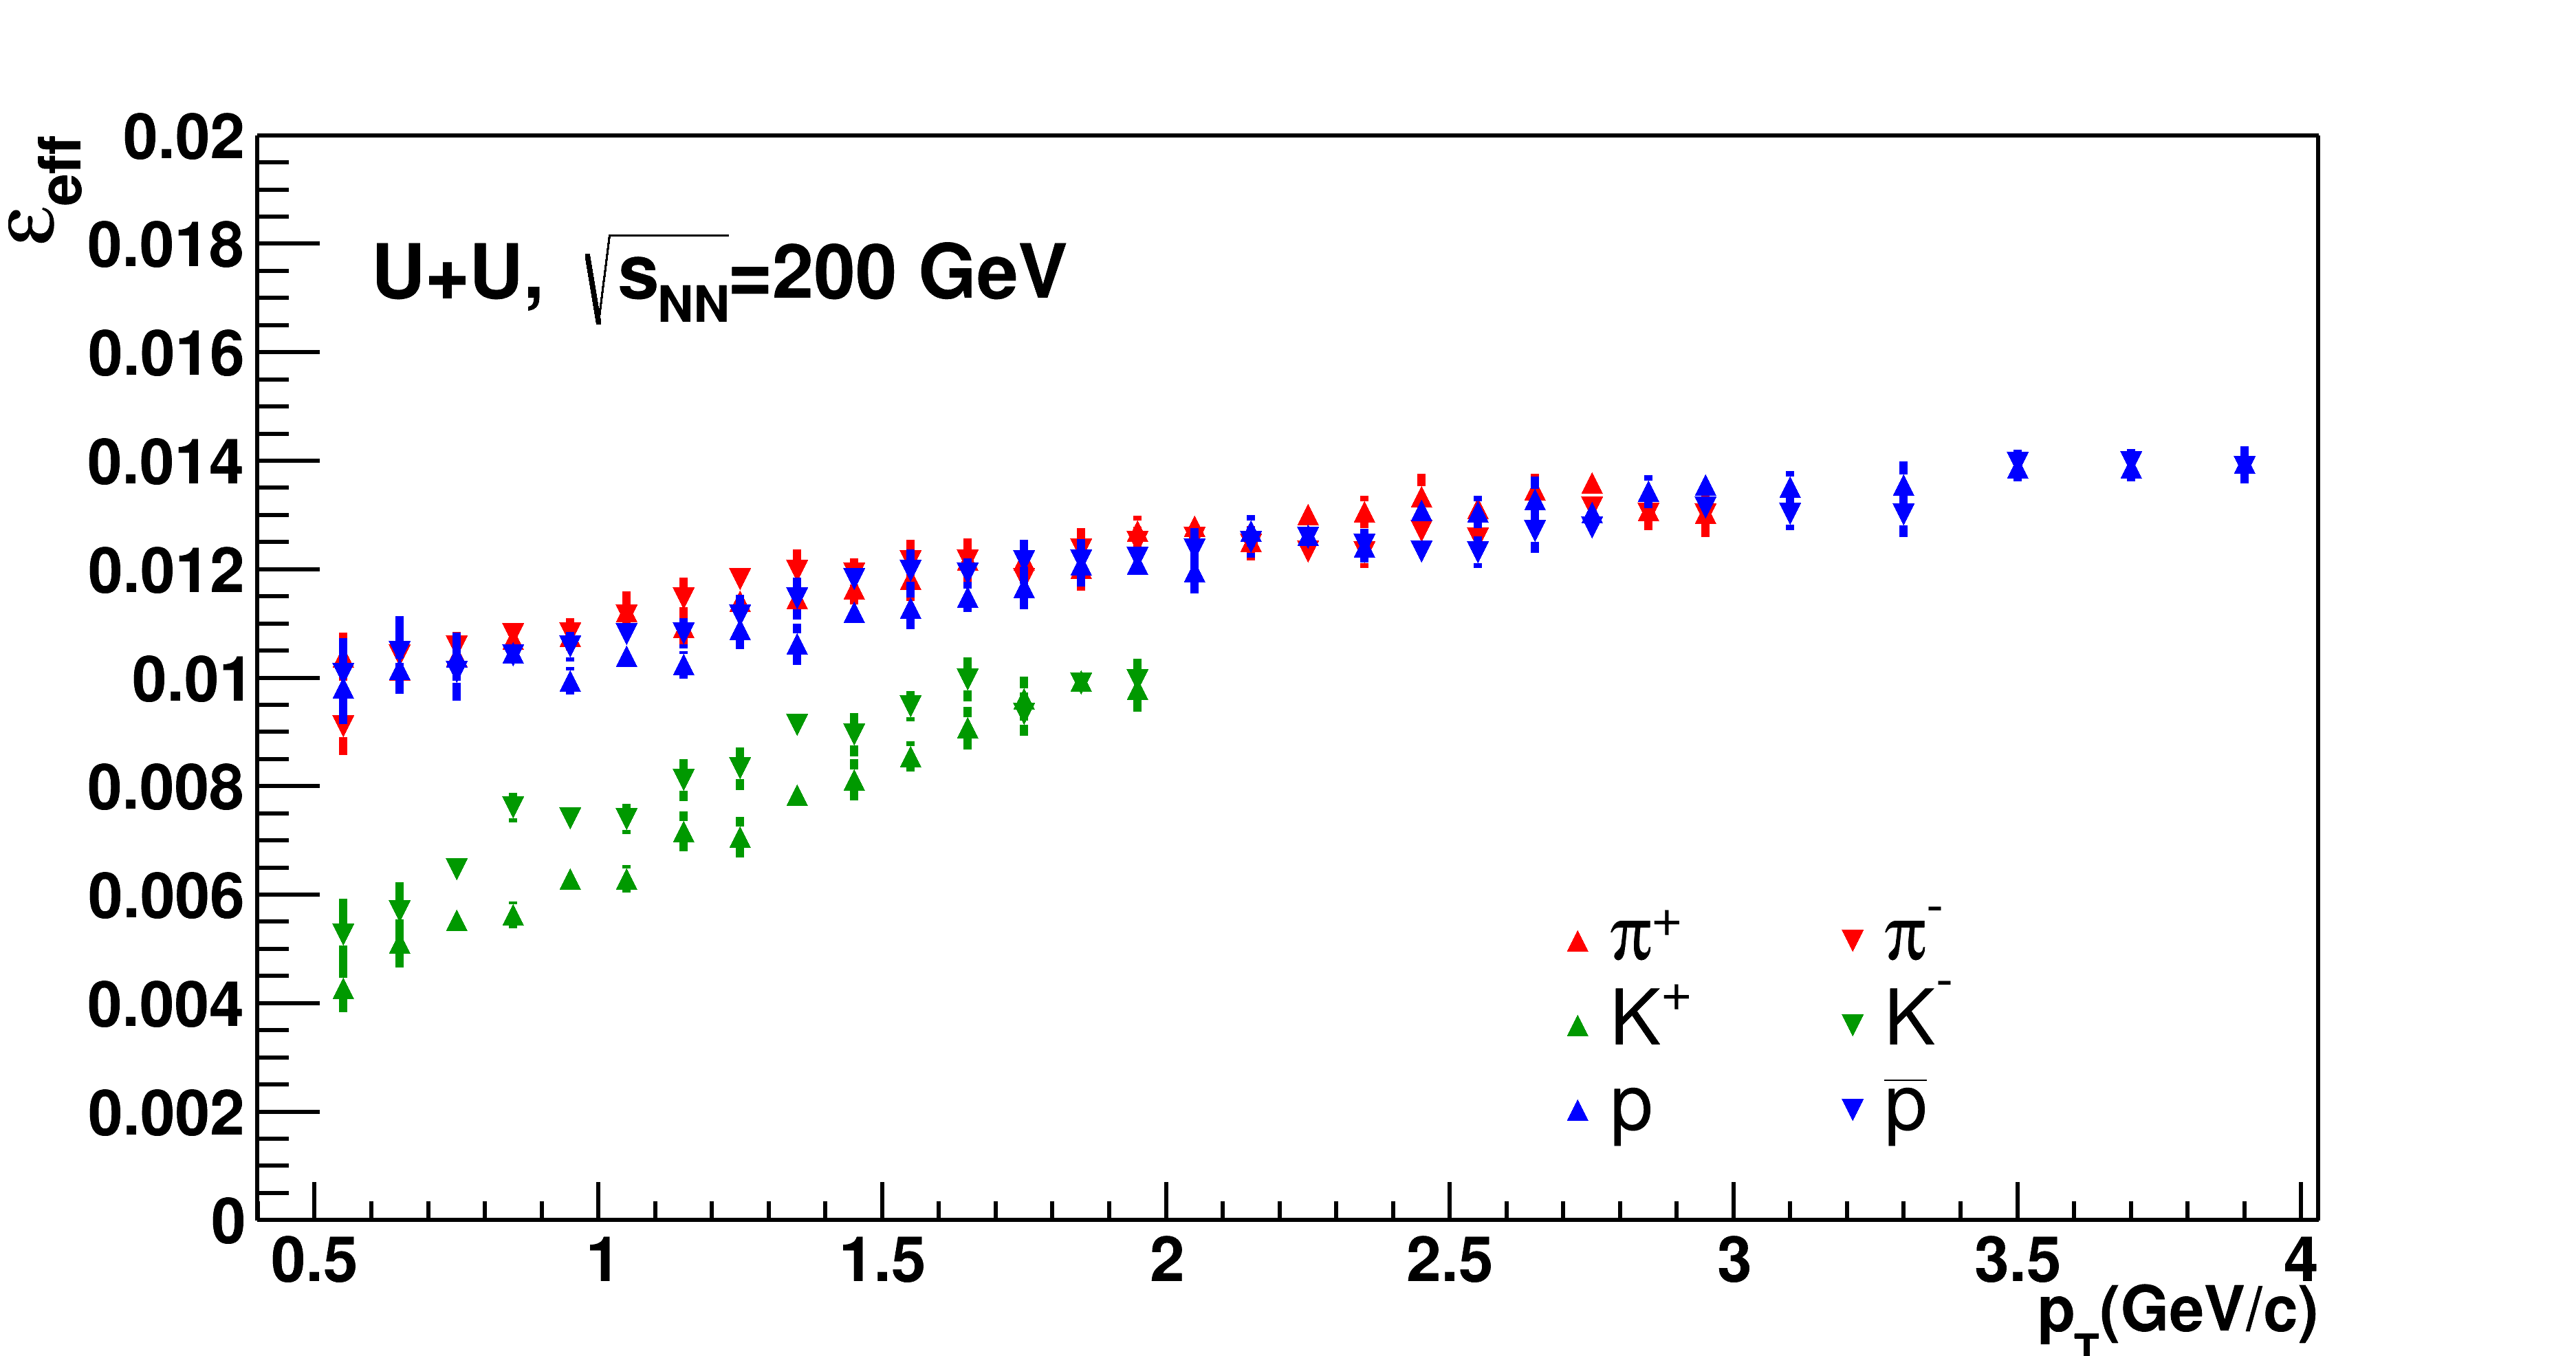
\includegraphics [width=0.9\linewidth]{Methodology/eff_hadron_UU.png}
	\caption{Эффективность регистрации заряженных адронов в столкновениях U+U.} 
	\label{img:eff_UU}
\end{figure}

%====================================================================================

\begin{figure}[] 
	\centerfloat
	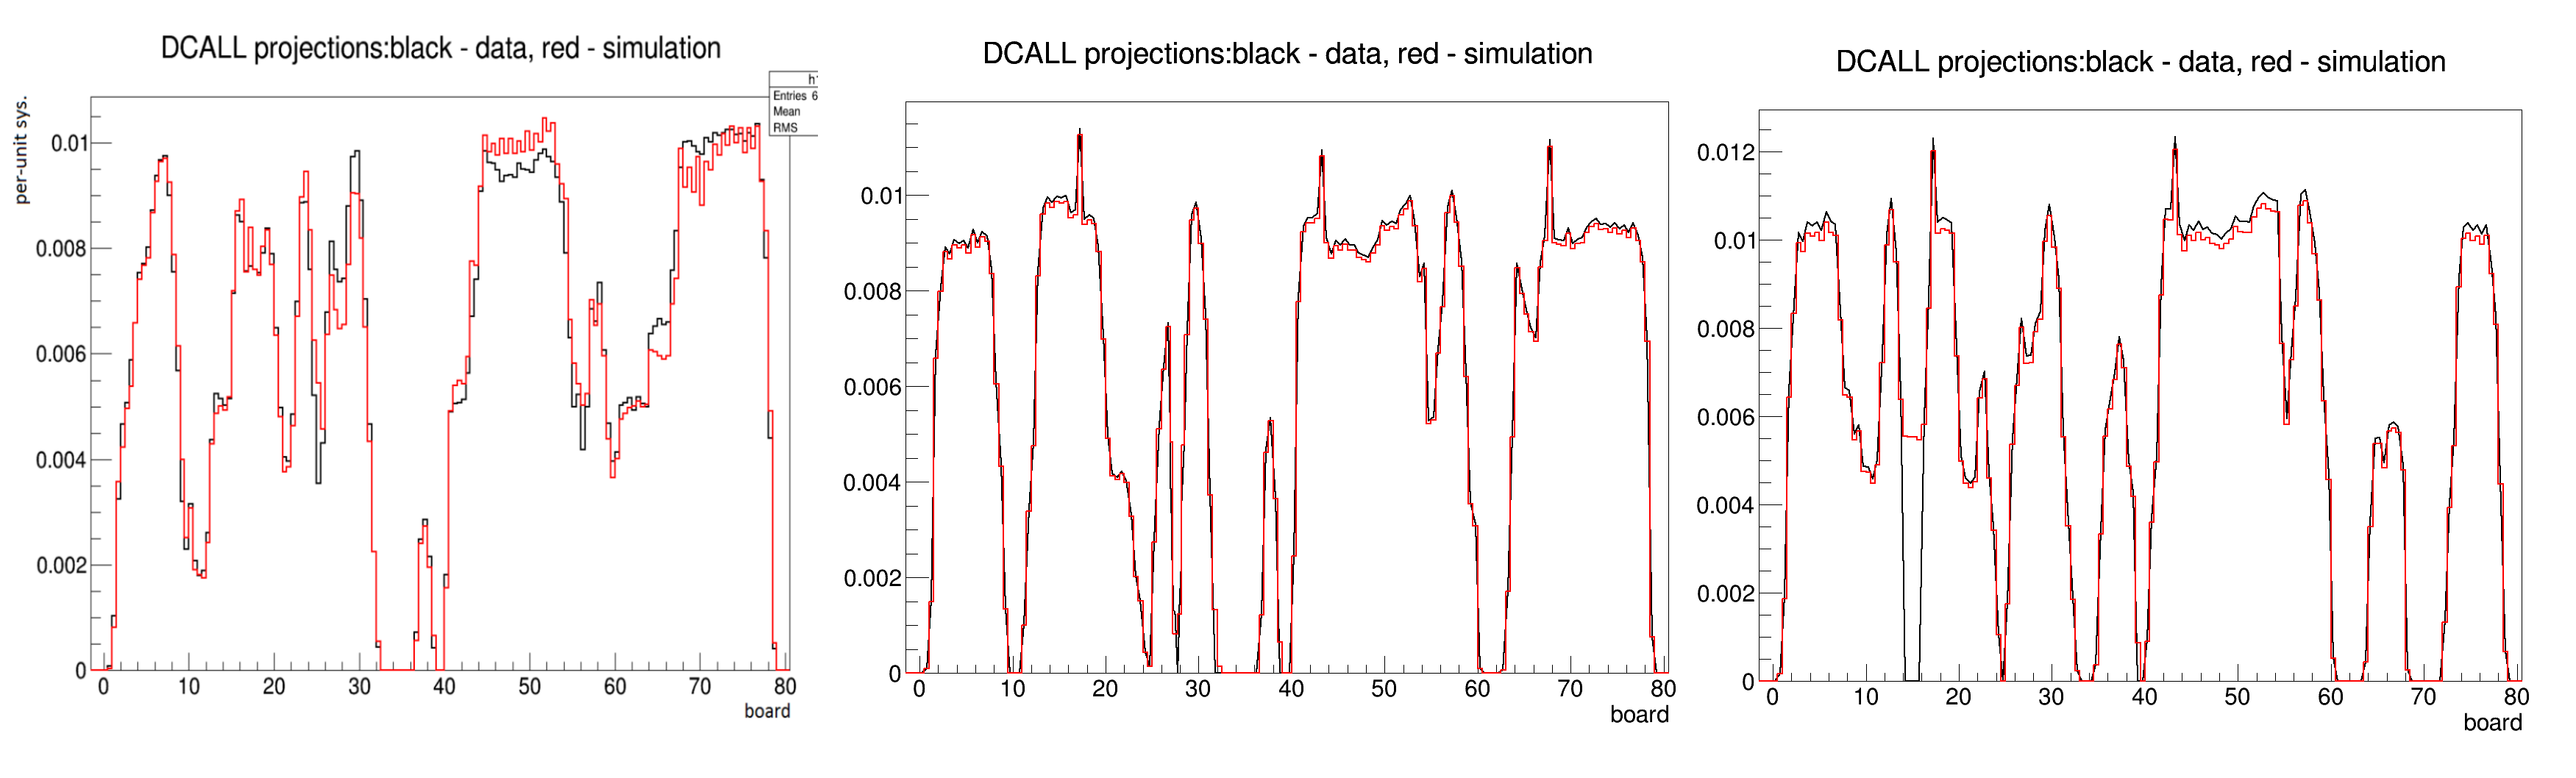
\includegraphics [width=\linewidth]{Methodology/DC_compar.png}
	\caption{Гистограммы распределения треков в зависимости от номера <<платы>> ДК, полученные путем моделирования и на основе экспериментальных данных в 2012г, 2014г и 2015г.} 
	\label{img:DC_compar}
\end{figure}

\begin{figure}[] 
	\centerfloat
	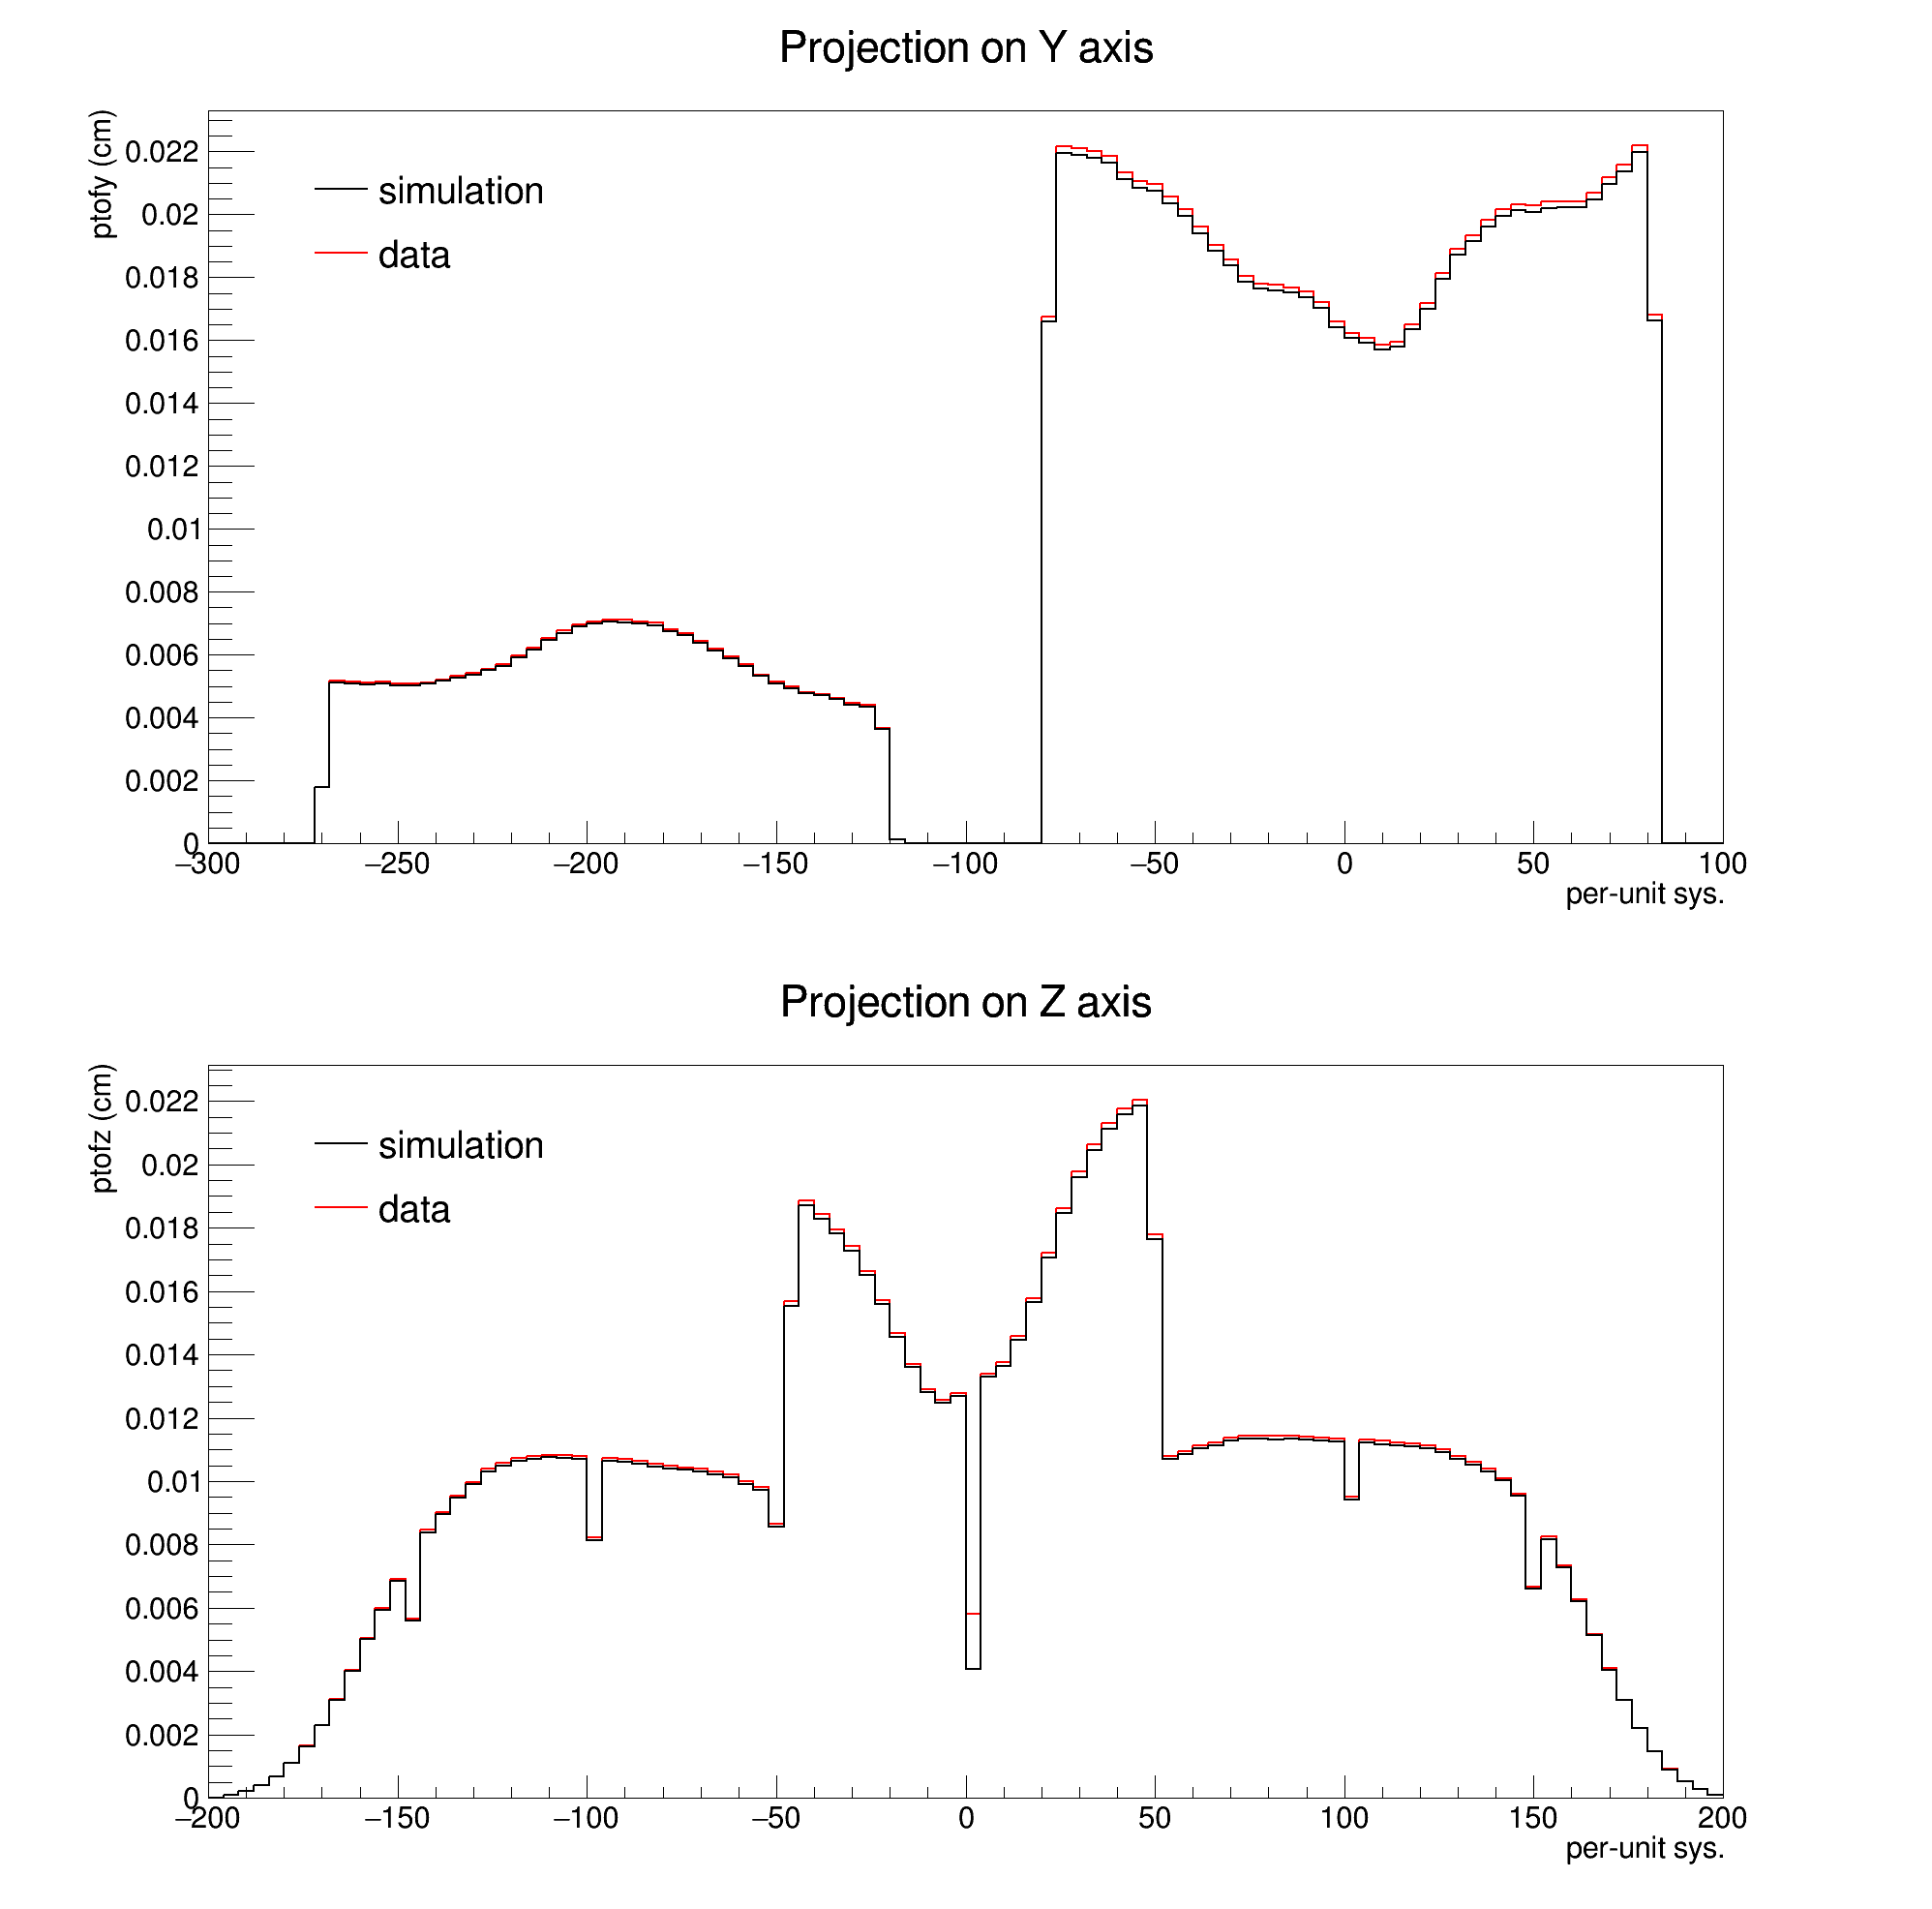
\includegraphics [width=0.9\linewidth]{Methodology/TOF_proj_pAl.png}
	\caption{Гистограммы распределения треков на плоскость $z-y$ детектора TOFE, полученные с использованием экспериментальных данных и данных моделирования 2015г. } 
	\label{img:TOFproj_pAl}
\end{figure}

\begin{figure}[] 
	\centerfloat
	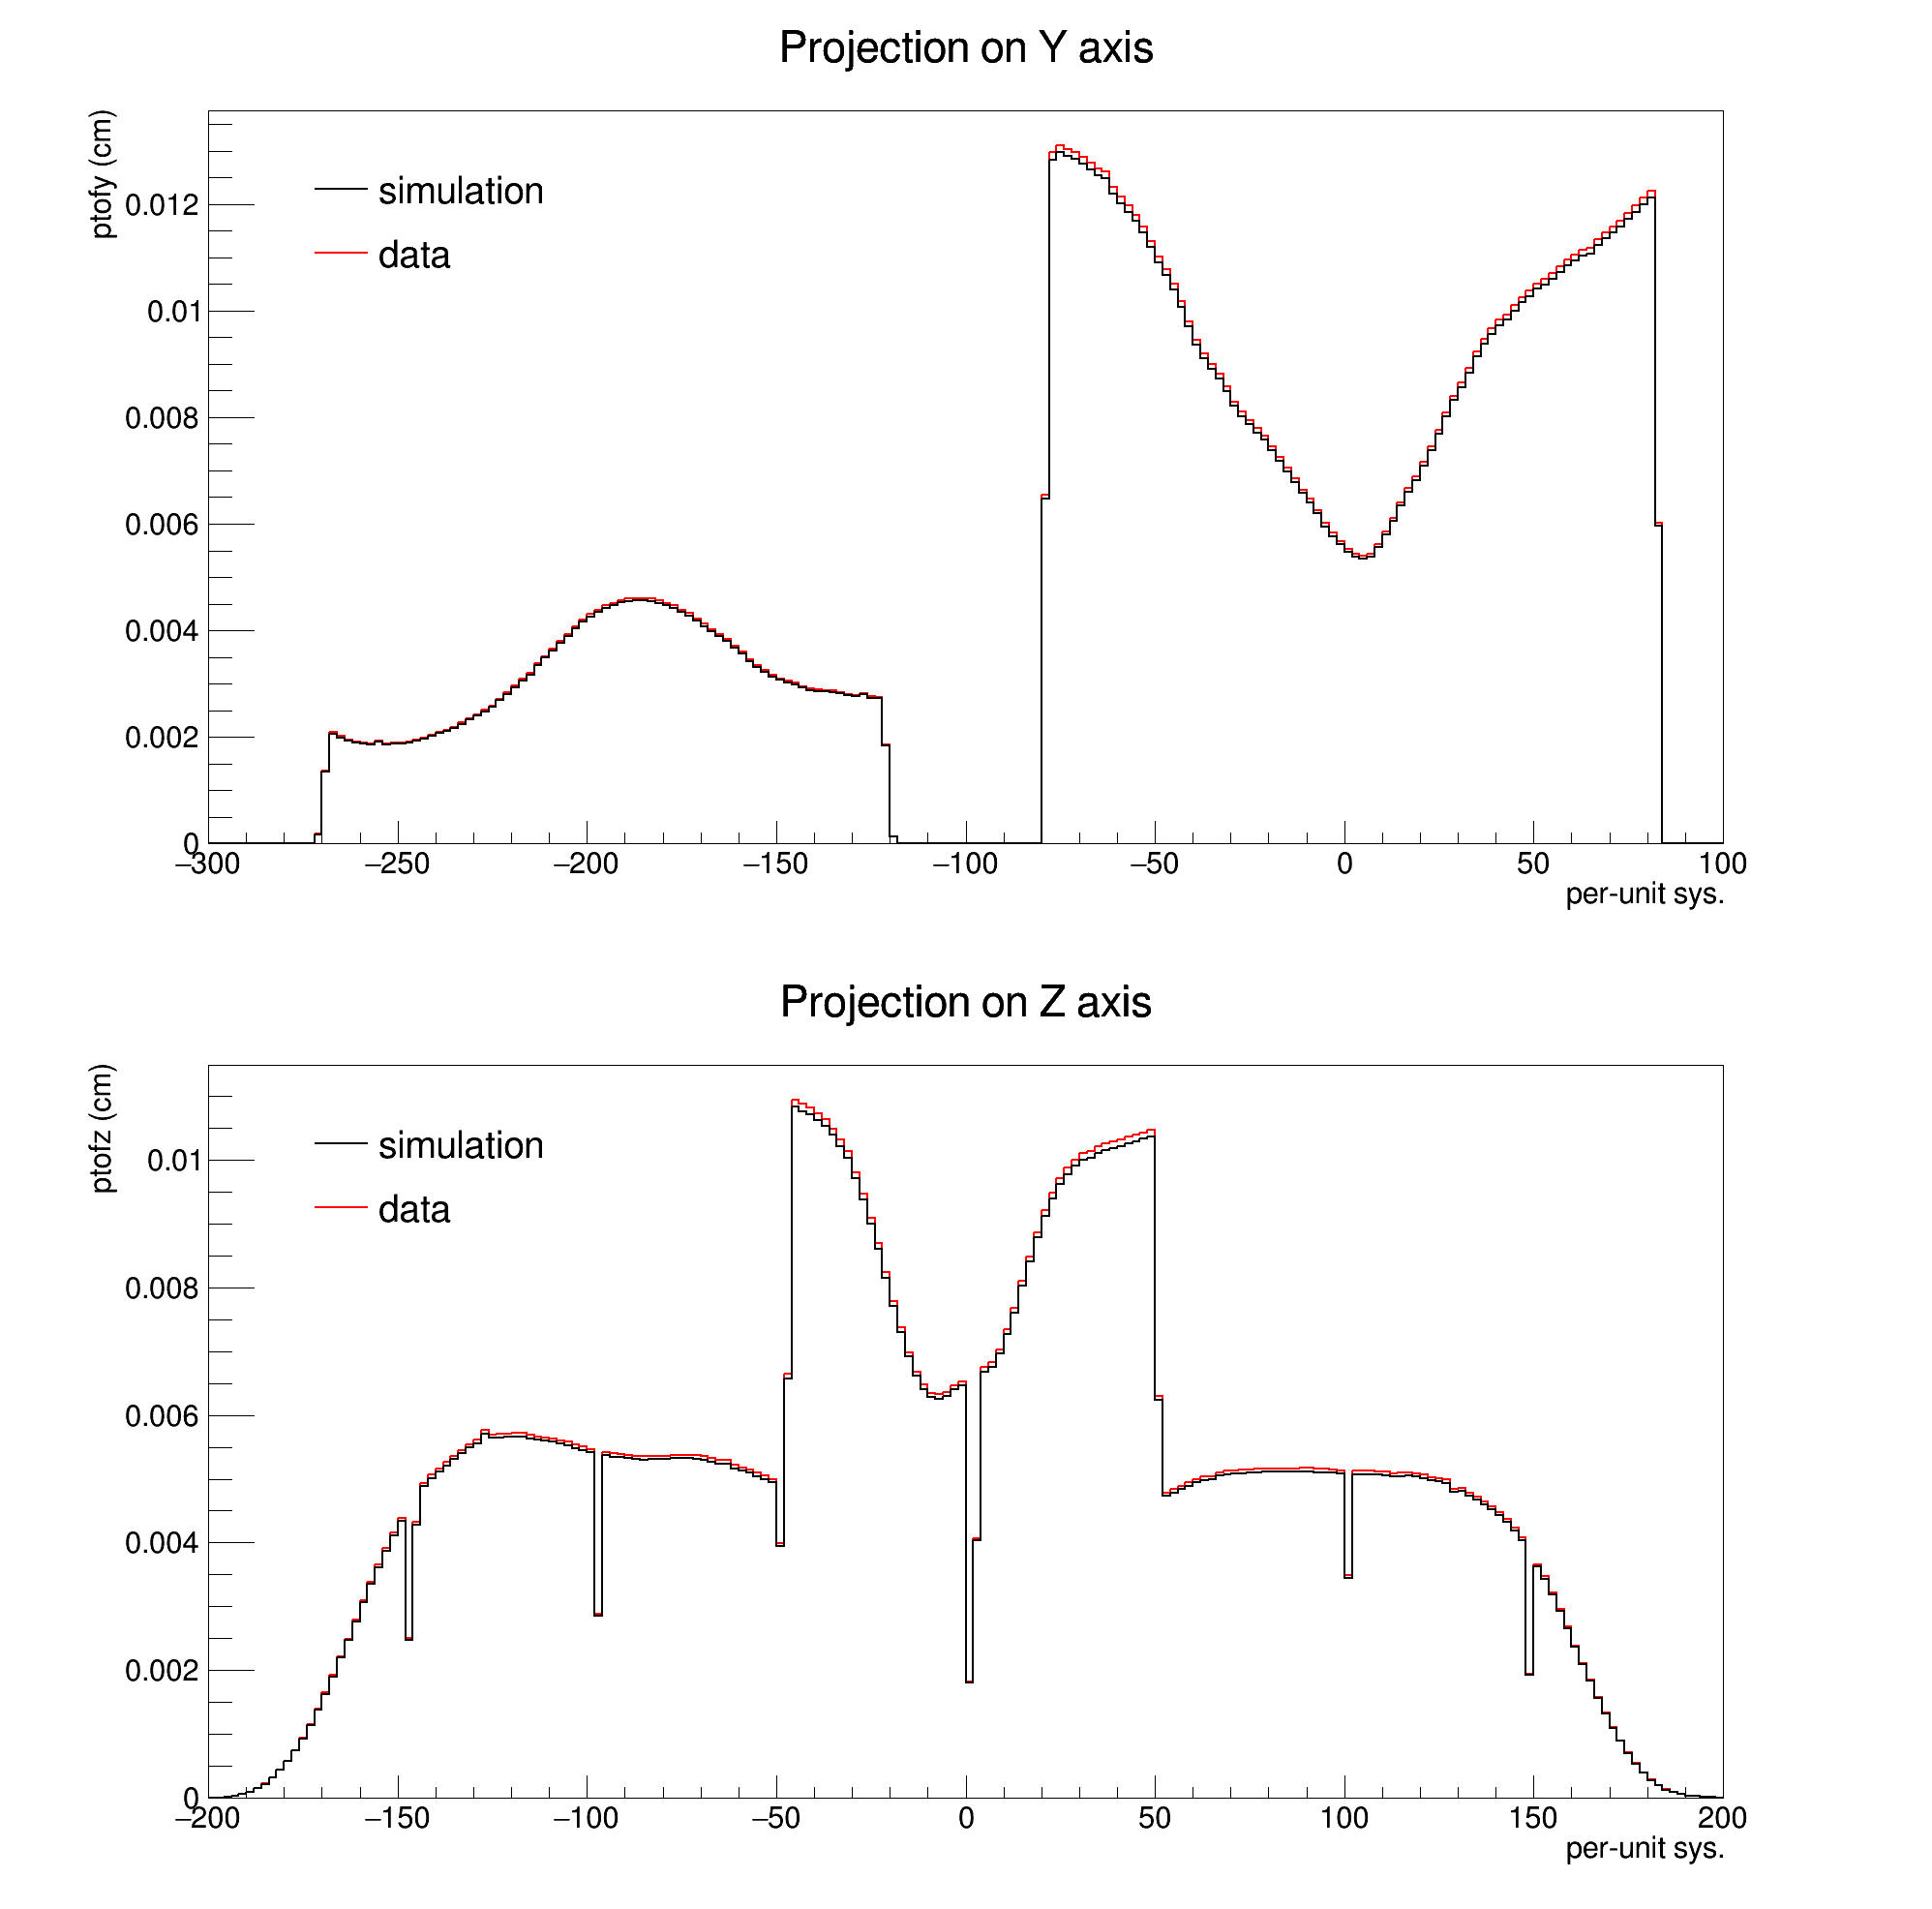
\includegraphics [width=0.9\linewidth]{Methodology/TOF_proj_HeAu.png}
	\caption{Гистограммы распределения треков на плоскость $z-y$ детектора TOFE, полученные с использованием экспериментальных данных и данных моделирования 2014г.} 
	\label{img:TOFproj_HeAu}
\end{figure}

\begin{figure}[] 
	\centerfloat
	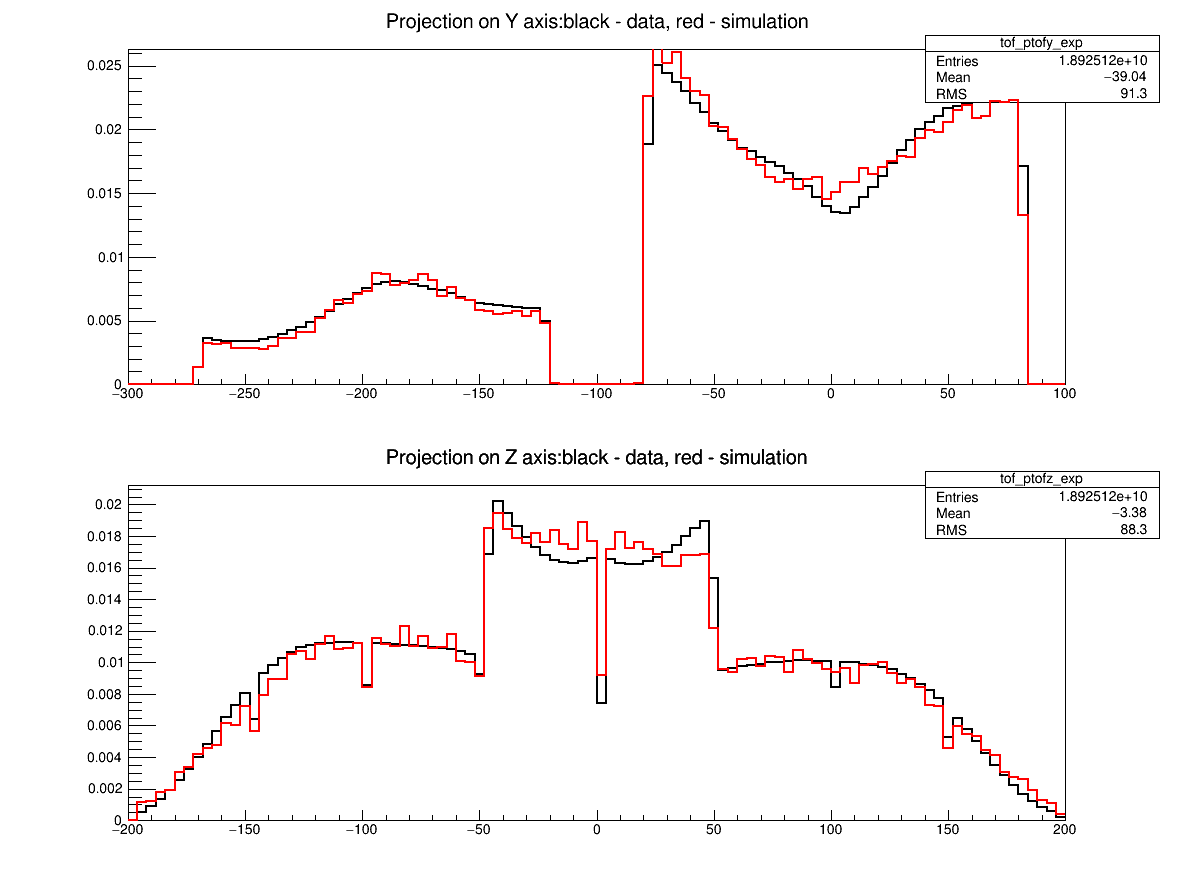
\includegraphics [width=0.9\linewidth]{Methodology/TOF_proj_CuAu.png}
	\caption{Гистограммы распределения треков на плоскость $z-y$ детектора TOFE, полученные с использованием экспериментальных данных и данных моделирования 2012г.} 
	\label{img:TOFproj_CuAu}
\end{figure}

\begin{comment}
\begin{figure}[] 
	\centerfloat
	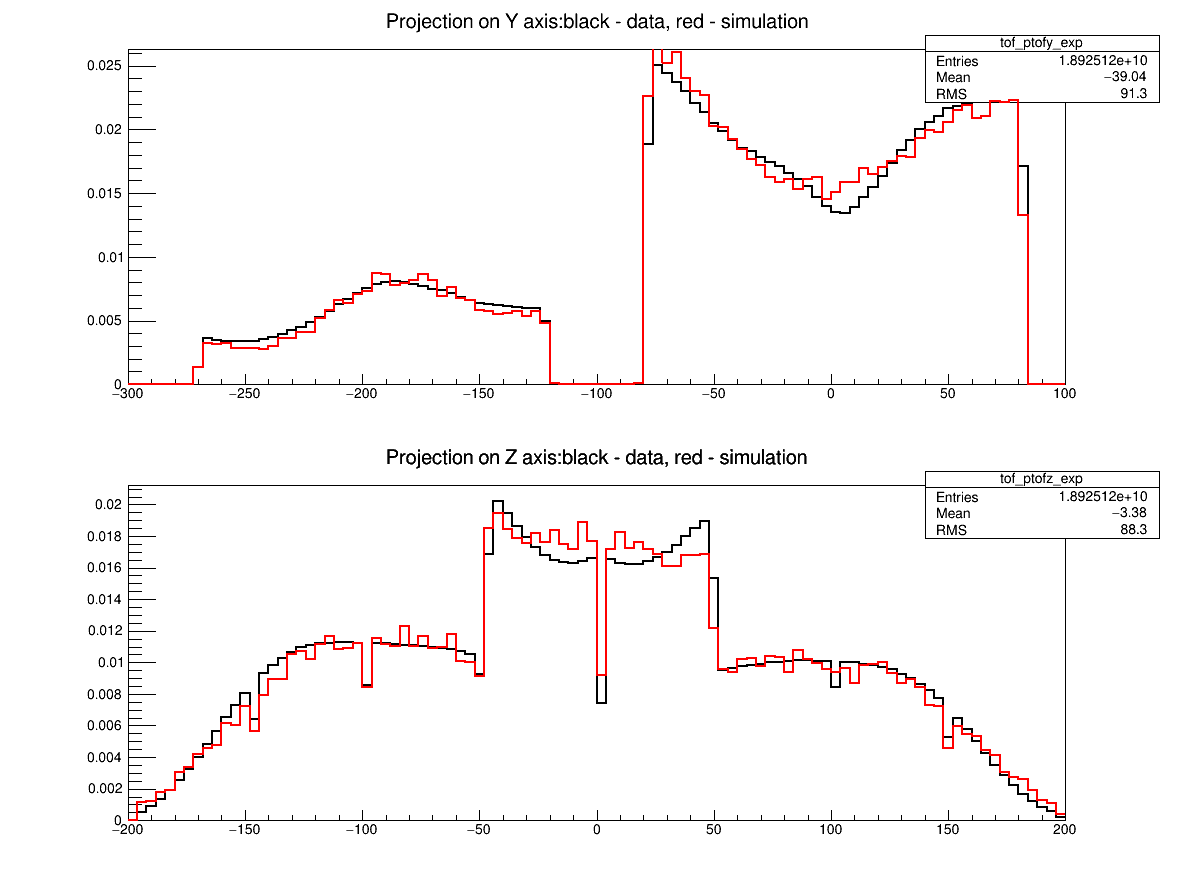
\includegraphics [width=0.9\linewidth]{Methodology/TOF_proj_UU.png}
	\caption{TOFproj U+U.} 
	\label{img:TOFproj_UU}
\end{figure}
\end{comment}

\subsection{Коррекция вклада слабых распадов} \label{sect3:FeedDown}
%Weak Decay Correction - поправка слабого взаимодействия
Для оценки количества протонов, родившихся непосредственно столкновении релятивистских ядер, была введена поправка $C_{FD}$, учитывающая образование протонов в результате слабых распадов. Поскольку наибольший вклад в образование протонов вносят $\Lambda$-барионы, фактор $C_{FD}$ в данной работе был вычислен как процент протонов, образовавшихся в результате распада $\Lambda$-барионов ($N_{\Lambda}^p$), от общей выборки протонов ($N_{tot}^p$ ):
\begin{equation}
	\label{eq:Lambda_pT}
	C_{FD} = \frac{N_{\Lambda}^p}{N_{tot}^p}.
\end{equation}

Для оценки величины $C_{FD}$ было проведено Монте-Карло моделирование рождения $\Lambda$-барионов, с теми же параметрами, которые были использованы для моделирования протонов. Для учета зависимости спектров $\Lambda$-барионов от поперечного импульса, гистограммы были взвешены с весом, вычисляемым по формуле \ref{eq:Lambda_pT}:
\begin{equation}
	\label{eq:Lambda_pT}
	W(p_{T}) = p_{T} e^{\frac{m_T-m_0}{T}}.
\end{equation}
Данная форма выбрана для наиболее точного представления $\Lambda$ и спектра протонов.
Затем в эту долю вносят поправку на коэффициент ветвления и отношения выходов $\Lambda$-барионов к протонам.
% Были использованы следующие значения отношений $\Lambda/p$:

Измерения $\Lambda$-барионов автоматически учитывают распады $\Sigma^0$-барионов, поскольку $\Sigma^0$-барионы  электромагнитно распадаются на $\Lambda$ и фотоны с коэффициентом ветвления 100 \%. В данной работе не было учтено рождение протонов в других распадах, таких как распады заряженных состояний $\Sigma$-барионов, а также многостранных барионных состояний $\Xi$ и $\Omega$. 

Систематическая неопределенность процента протонов, образовавшихся в результате распада $\Lambda$-барионов, от общей выборки протонов оценивается в 25 \%, что в первую очередь связано с неопределенностью величины отношения $\Lambda/p$. Доля распадных протонов составляет порядка 10–40\%, поэтому изменение отношения $\Lambda /p$ на 25\% приводит к изменению спектра протонов примерно на 2,5–10\%.
На Рисунке \ref{img:FeedDown} показана зависимость доли распадных протонов и антипротонов от поперечного импульса. 

\begin{figure}[] 
	\centerfloat
	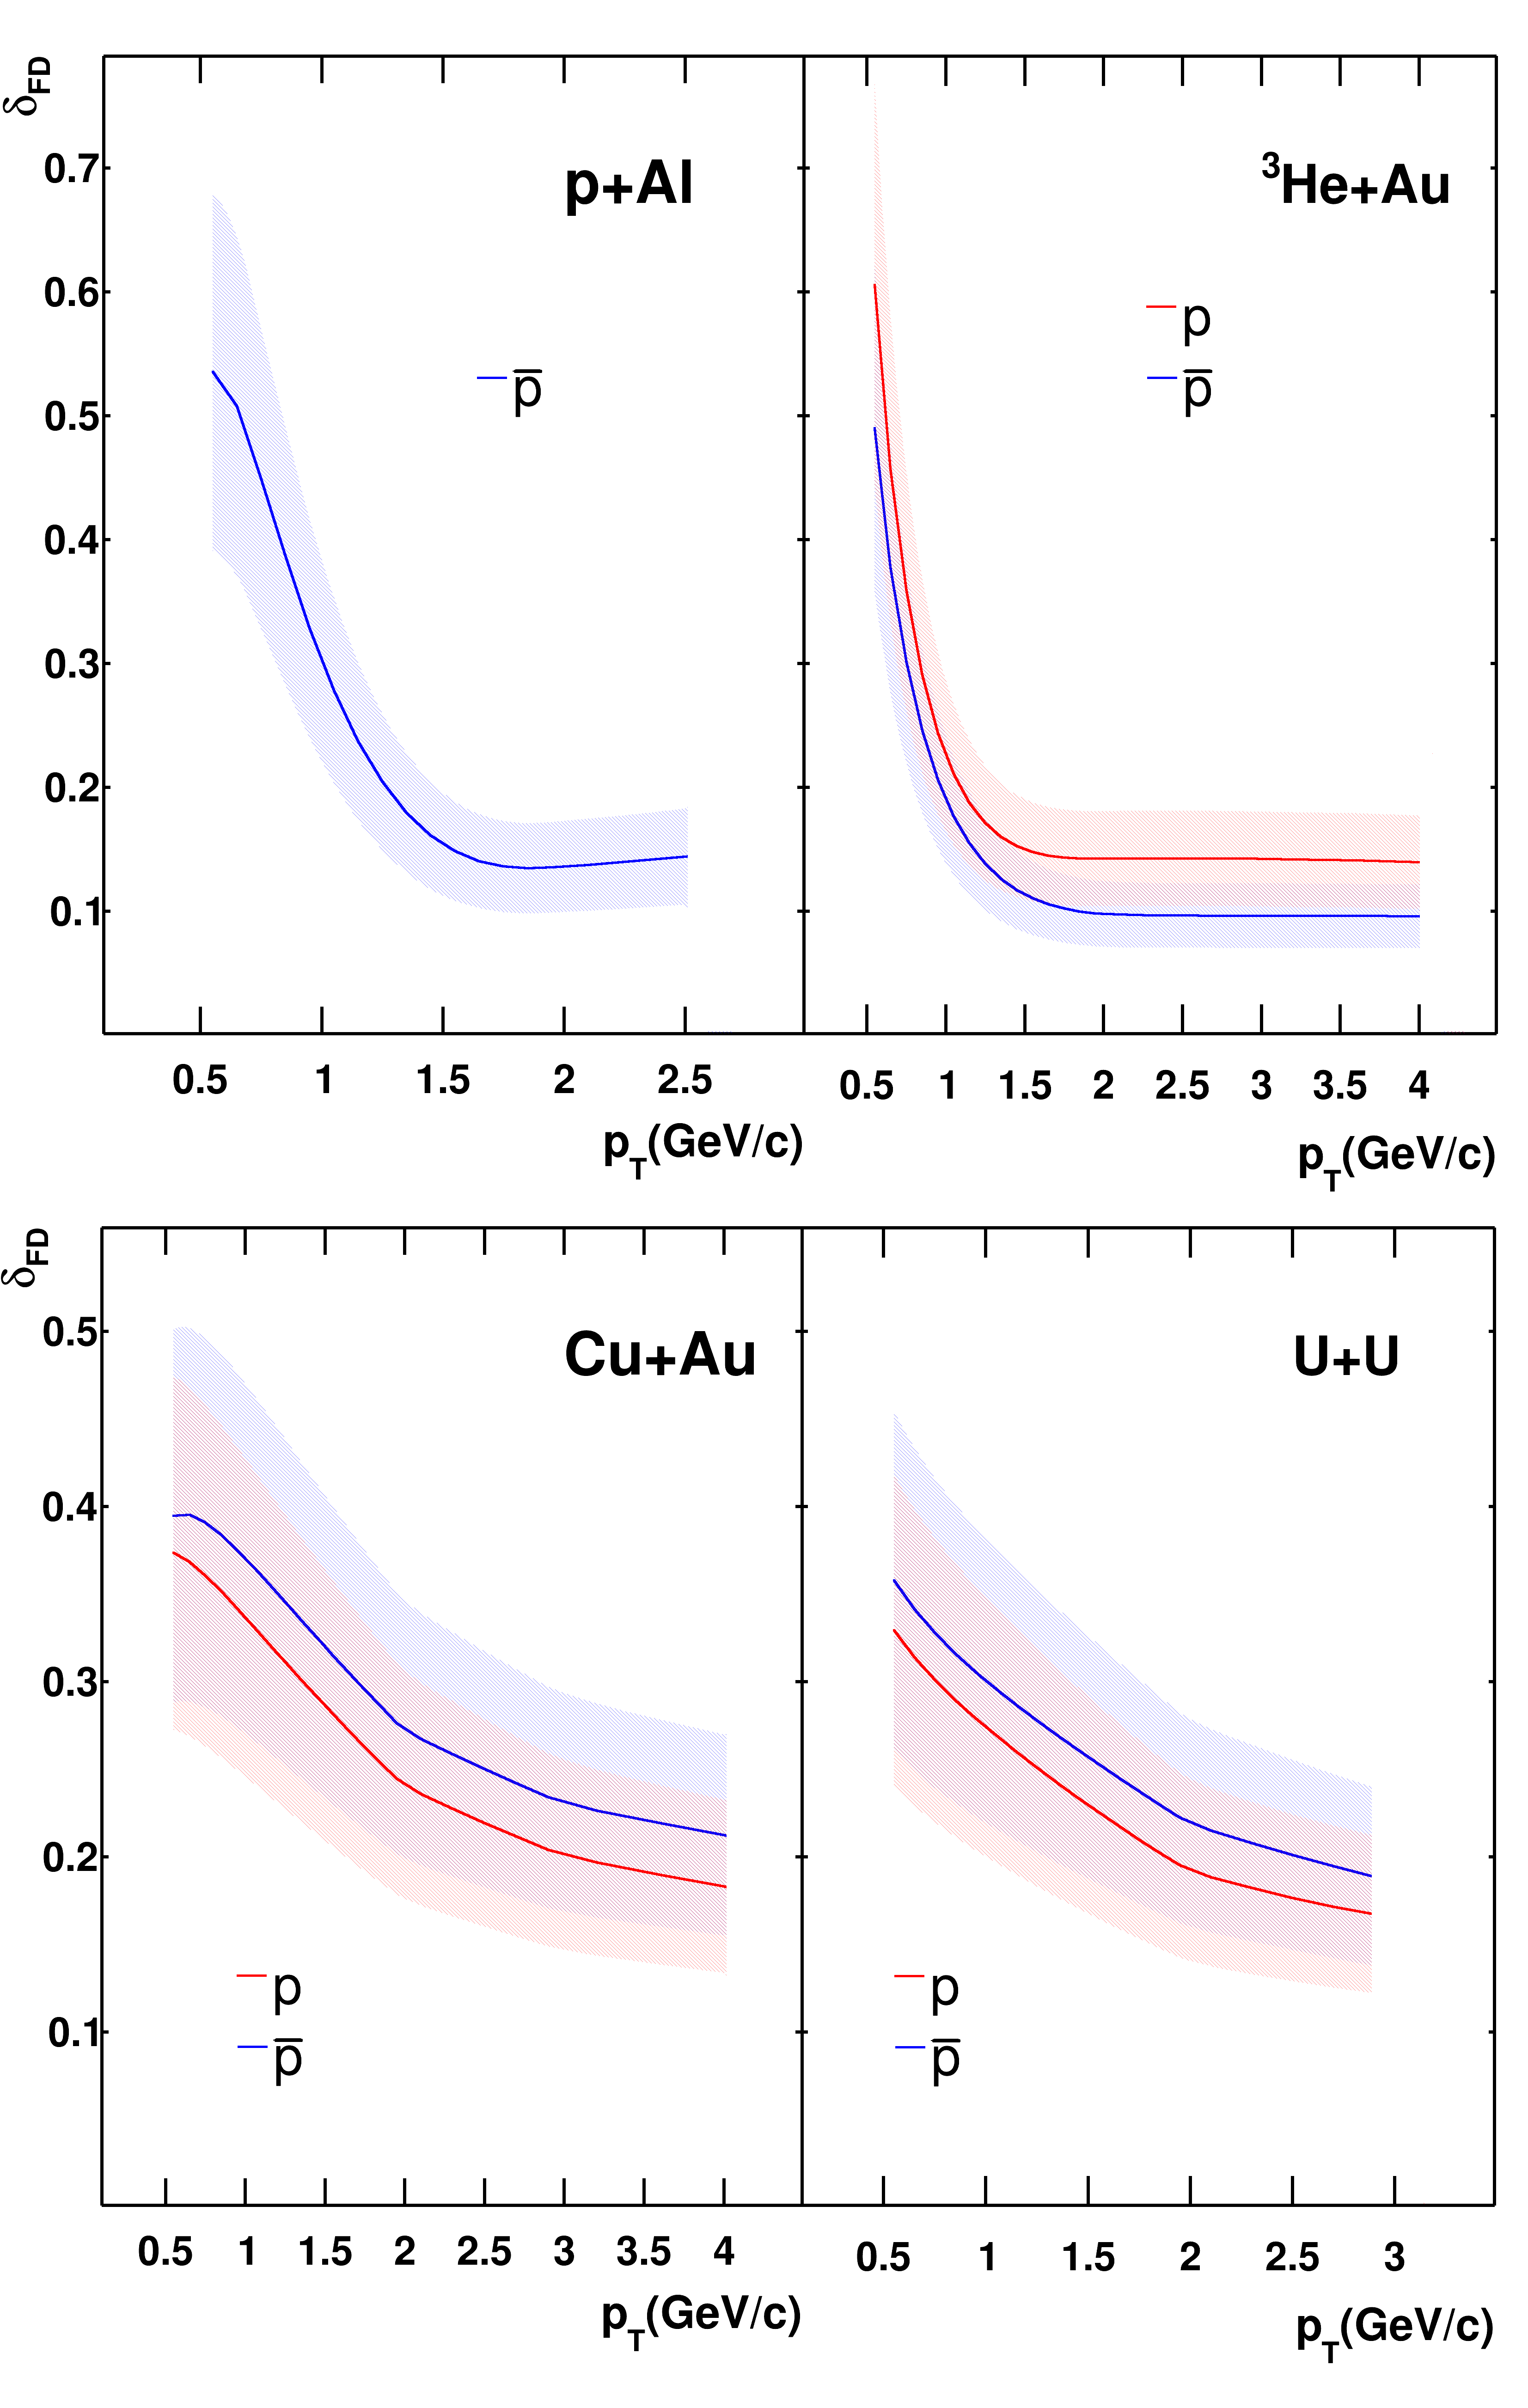
\includegraphics [width=0.7\linewidth]{Methodology/FeedDown.png}
	\caption{Значения $C_{FD}$, вычисленные в \pal, \heau, Cu+Au, U+U  столкновениях. Заштрихованные области обозначают систематические погрешности.} 
	\label{img:FeedDown}
\end{figure}

\section{Систематические неопределенности} \label{sect3:Syst}
В данном разделе приведены оценки статистических и  систематических погрешностей измерений. 
Статистическая погрешность измерений определяется объемом используемой выборки данных. 
Систематические погрешности отражают неопределенности, не связанные с количеством измерений, а обусловленные произвольным выбором параметров анализа. 

% В данном разделе приведены классификация систематических неопределенностей (п. \ref{sect3:SystClass}), описаны источники систематической неопределенности (п. \ref{sect3:SystSource}) и приведены результаты оценки систематической неопределенности (п. \ref{sect3:SystValues}).

%\subsection{Классификация неопределенностей измерений} \label{sect3:SystClass}
 %Методика определения статистической неопределенности измерения выходов заряженных адронов приведена в п. \ref{sect3:SystValues}. По своей природе, величина статистической неопределенности не коррелирована по поперечному импульсу и центральности.
Систематические погрешности принято разделять на три вида: А, B и C.
Неопределенность <<типа A>> описывает ошибки измерений, некоррелированные по поперечному импульсу. То есть неопределенность <<типа A>> сдвигает значения, измеренные при различных \pt, на различные произвольные некоррелированные величины. 
Неопределенность <<типа B>> описывает ошибки измерений, которые определенным образом зависят от величины поперечного импульса, однако точный вид данной зависимости не известен. 
Неопределенность <<типа C>> определяется ошибками измерений, которые одинаковы во всем диапазоне поперечных импульсов. Таким образом, неопределенность <<типа C>> как бы сдвигает все измеренные значения одновременно во всем диапазоне \pt. В данной работе неопределенность типа C обусловлена неопределенностью измерения значений \Ncoll.

В данной работе отдельно выделяется неопределенность типа <<C>>, а неопределенности типа <<A>> и <<B>> суммированы. Суммарные неопределенности типа <<A>> и <<B>> далее изображаются прямоугольниками вокруг точек на графиках, а неопределенность типа <<C>> изображается прямоугольником вдоль оси \pt, отражая ее общность для всех точек на графике. 

\subsection{Источники систематических неопределенностей измерения заряженных адронов} \label{sect3:SystSource}
Как было указано ранее, систематические погрешности отражают неопределенности, не связанные с количеством измерений, а обусловленные произвольным выбором параметров анализа. Ниже перечислены такие произвольные параметры данной работы, а также описаны систематические неопределенности, им соответствующие.

\bfseries Неопределенности, связанные с исключением мертвых областей дрейфовой камеры. %DC fiducial
\mdseries
Данная систематическая неопределенность связана с произвольностью определения границ мертвых областей исключаемых из дальнейшего рассмотрения. Для оценки величины такой неопределенности, было проведено сравнение значений первичных выходов заряженных адронов, измеренных стандартным способом, а также двумя альтернативными способами: без  исключения мертвых областей дрейфовой камеры, а также с исключением мертвых областей, уменьшенных на 5 мрад по сравнению со стандартным методом. 
Результаты оценки данной систематической неопределенности представлены в Таблице \ref{table:systDCFiduciual} Приложения \ref{app:A}.


\bfseries Неопределенность, связанная с ограничением $z$-координаты трека частицы в ДК ($zed$) при отборе событий. % DC zed
\mdseries
Для оценки неопределенности, связанной с ограничением $z$-координаты трека частицы в ДК ($zed$) при отборе событий, проводится сравнение результатов измерения заряженных адронов со стандартным критерием отбора данных $|zed|<75$ и измерения заряженных адронов, с условием $|zed|<40$. 
Результаты оценки данной систематической неопределенности представлены в Таблице \ref{table:systDCZed} Приложения \ref{app:A}.

\bfseries Неопределенность идентификации частиц во времяпролетной камере.
\mdseries
вызвана погрешностью определения параметров функции \ref{eq:TOFgaus_approx} и значений  $\sigma_h$ и $m_h$ (п. \ref{sect3_PID}). Данная неопределенность была оценена путем сравнения первичных выходов заряженных адронов, идентифицированных согласно стандартным критериям, описанным в п. \ref{sect3_PID}, а также идентифицированных с использованием условий $ m^2_h -2,5\sigma_h < m^2 < m^2_h +2,5\sigma_h $ и  $ m^2_h -1,5\sigma_h < m^2 < m^2_h +1,5\sigma_h $.

\bfseries Неопределенность, связанная с ограниченным аксептансом дрейфовой камеры.
\mdseries
Систематическая неопределенность, связанная с неидеальностью воспроизведения геометрии электромагнитного калориметра в Монте-Карло модели, оценивалась по изменению отношения данных к результатам моделирования (см.  Рисунок \ref{img:DC_compar}). Это изменение было получено путем выбора различных областей для нормировки результатов моделирования на представление того же общего интеграла, что и в экспериментальных данных. Было выбрано 10 различных областей вдоль оси номеров плат ДК. Каждая область поочередно использовалась для нормировки распределений треков в ДК, полученных из экспериментальных данных и моделирования. Для каждой из 10 проведенных нормировок были вычислены отношения полных интегралов распределений треков в ДК, полученных из экспериментальных данных и моделирования. Итоговое значение рассматриваемой погрешности было вычислено как среднеквадратичное значение отношения 10 полученных данных к интегралам моделирования. 

\subsection{Значения систематических неопределенностей спектров заряженных адронов} \label{sect3:SystValues}
Полученные значения систематических неопределенностей измерений выходов идентифицируемых заряженных адронов для каждого из перечисленных в п.\ref{sect3:SystSource} источника, приведены в Таблицах \ref{table:systDCFiduciual}-\ref{table:systPID} Приложения \ref{app:A}.
Считая вклады неопределенностей различных типов некоррелированными, итоговые значения систематических погрешностей вычислялись как  среднеквадратическое значение величин неопределенностей различных типов. Полученные итоговые значения систематических неопределенностей приведены в Таблице \ref{table:systTotal}.
Наибольший вклад в суммарные значения систематических неопределенностей  измерения выходов заряженных адронов являются неопределенности, вносят неопределенности, связанные с исключением мертвых областей дрейфовой камеры и идентификации частиц во времяпролетной камере, относительная величина которых увеличивается от 2 до 9\% с ростом поперечного импульса. 

\begin{table}[]
	\caption{Итоговые значения систематических неопределенностей измерений (\%) заряженных адронов}
	\label{table:systTotal}
	
	\begin{tabularx}{\linewidth}
		{ 
			| >{\raggedright\arraybackslash}X 
			| >{\centering\arraybackslash}X 
			| >{\centering\arraybackslash}X 
			| >{\centering\arraybackslash}X 
			| >{\centering\arraybackslash}X 
			| >{\centering\arraybackslash}X 
			| >{\centering\arraybackslash}X | }
		\hline
	Система &\pt (ГэВ/$c$) 
	&  0,5 -- 1,0 & 1,0 -- 1,5 & 1,5 -- 2,0 & 2,0 -- 3,0 &  3,0 -- 4,0  \\ \hline
		\multirow{6}{*}{\pal}  
	& \pip & 9,7 & 10,5 & 11,3 & 11,2 & --   \\ \cline{2-7} 
	& \pim & 8,7 & 11 & 10,5 & 10,1 & --   \\ \cline{2-7} 
	& \Kp & 7,9 & 10,2 & 13,7 & --& --   \\ \cline{2-7} 
	& \Km & 7,7 & 9,9 & 15 & --& --   \\ \cline{2-7} 
	& \prot & 10,3 & 11,5 & 12,4 & 13,1 & 16,5    \\ \cline{2-7} 
	& \aprot & 8,4 & 8,6 & 10,3 & 10,9 & 12,8    \\
	 \hline \hline
	\multirow{6}{*}{\heau}
	& \pip & 5,7 & 4,2 & 5,7 & 6,7 & --   \\ \cline{2-7} 
	& \pim & 11,6 & 11,3 & 10,5 & 9,1 & --   \\ \cline{2-7} 
	& \Kp & 8,3 & 8,6 & 10 & --& --   \\ \cline{2-7} 
	& \Km & 8,7 & 9,9 & 11,3 & --& --   \\ \cline{2-7} 
	& \prot & 8,6 & 8,6 & 8,8 & 8,5 & 8,8    \\ \cline{2-7} 
	& \aprot & 9,1 & 10 & 10,4 & 10,3 & 10,6    \\ 
	 \hline \hline
	\multirow{6}{*}{Cu+Au}
	& \pip & 10,2 & 10,9 & 10,5 & 9,9 & --   \\ \cline{2-7} 
	& \pim & 8,9 & 10,1 & 10 & 10,5 & --   \\ \cline{2-7} 
	& \Kp & 10,2 & 8,3 & 7,5 & --& --   \\ \cline{2-7} 
	& \Km & 10 & 7,7 & 8,6 & --& --   \\ \cline{2-7} 
	& \prot & 9 & 9 & 9,7 & 11,3 & 11,1    \\ \cline{2-7} 
	& \aprot & 9,3 & 7,9 & 7,7 & 8,8 & 8,9    \\ \hline \hline
	\multirow{6}{*}{U+U}
	& \pip & 16,8 & 16,5 & 14,7 & 13,7 & --   \\ \cline{2-7} 
	& \pim & 6,2 & 8,8 & 9,4 & 16,9 & --   \\ \cline{2-7} 
	& \Kp & 10,2 & 8,3 & 8,3 & --& --   \\ \cline{2-7} 
	& \Km & 8,8 & 7,6 & 8,5 & --& --   \\ \cline{2-7} 
	& \prot & 10 & 9,8 & 9,8 & 11,2 & --   \\ \cline{2-7} 
	& \aprot & 10,3 & 10 & 9,1 & 10,5 & --    \\ \hline
		
	\end{tabularx}
\end{table}

\section{Инвариантные спектры по поперечному импульсу} \label{sectRes_spectra}
Для понимания адронно-адронных столкновений высоких энергий Ферми предложил следующий статистический метод \cite{ThermalModel}. Из-за насыщения фазового пространства рождение множества частиц в результате элементарных столкновений высоких энергий согласуется с тепловым описанием \cite{Thermal1, Thermal2, ThermalModel}. В столкновениях тяжелых ионов можно ожидать гидродинамического поведения, то есть локального теплового равновесия и коллективного движения из-за большого числа вторичных рассеяний. Адроны в конечном состоянии являются наиболее многочисленным и доминирующим источником информации о ранней стадии столкновений. Спектры адронов по поперечному импульсу и быстроте зависят от температуры и параметров коллективного потока частиц. Отношения спектров частиц чувствительны к химическим свойствам системы и механизму образования частиц.
% Недавний обзор существующих данных, полученных в основном из CERN-SPS, можно найти в литературе [10].

Измерение инвариантных спектров по поперечному импульсу является одним из основных инструментов для изучения рождения частиц в столкновениях релятивистских ионов.
Инвариантные спектры по поперечному импульсу вычисляются согласно формуле \ref{eq:pTspectra}:
\begin{equation}
	\label{eq:pTspectra}
	\frac{1}{2\pi p_T} \frac{d^2 N}{dp_T dy}=\frac{1}{2\pi p_T}\frac{N_h}{N_{evt} \varepsilon_{eff} \Delta p_T \Delta y},
\end{equation}
где $\Delta p_T$ – диапазон поперечных импульсов,

$\Delta y$ – диапазон быстрот, 

$N_h$ -- количество заряженных адронов $h$, зарегистрированных в диапазонах  $\Delta p_T, \Delta y$,  

$\varepsilon_{eff}$ -- эффективность регистрации адронов $h$.

Инвариантные спектры по поперечному импульсу связаны с распределением по инвариантной массе следующим образом:
\begin{equation}
	\label{eq:mTspectra}
	\begin{split}
		\frac{1}{2\pi p_T} \frac{d^2 N}{dp_T dy}=
		\frac{1}{2\pi \sqrt{m_T^2-m_0^2}} \frac{d^2 N}{d(\sqrt{m_T^2-m_0^2})dy}=\\
		\frac{1}{2\pi \sqrt{m_T^2-m_0^2}} \frac{d^2 N \sqrt{m_T^2-m_0^2}}{m_T dm_Tdy}=\frac{1}{2\pi m_T} \frac{d^2 N}{dm_Tdy},
	\end{split}
\end{equation}
где $m_0$ - масса адрона, $m_T = \sqrt{p_{T}^{2}+m_0^2}$.


Согласно моделям термодинамики \cite{Thermal1, Thermal2} в области $m_T<$1,5 ГэВ/с спектры имеют экспоненциальную форму и могут быть описаны  зависимостью \ref{eq:mTspectraEXP}:
\begin{equation}
	\label{eq:mTspectraEXP}
	\frac{1}{2\pi m_T} \frac{d^2 N}{dm_T dy}=\frac{1}{2\pi T (T+m_0)}\cdot A \cdot exp{\frac{-m_T -m_0}{T}},
\end{equation}
где $T$ - параметр обратного наклона спектра,

$A$ - нормировочный коэффициент, содержащий информацию о множественности рождения частиц в данном диапазоне быстрот $dN/dy$.
%В области \mt$>2$ ГэВ/с спектры начинают проявлять степенную зависимость от \mt. 

Параметр обратного наклона $T$ пропорционален средней поперечной кинетической энергии, следовательно, в рамках термодинамических моделей, проявляет следующую зависимость от массы адрона (см. раздел \ref{ch1/hydro}):
$$ T \sim T_{thermal}+m_0 \cdot \langle u_T ^2 \rangle.$$


\section{Факторы ядерной модификации}
Для количественного сравнения выходов адронов в ядро-ядерных и протон-протонных соударениях были вычислены факторы ядерной модификации (\rab). Для столкновений ядер A и B значение \rab \ определяется соотношением
\begin{equation}
	\label{eq:rab}
	R_{AB}=\frac{1}{N_{coll}}\frac{d^2 N_{A+B}/dp_T dy}{d^2 N_{p+p}/dp_T dy},
\end{equation}
где \Ncoll \ – количество парных нуклон-нуклонных соударений;
 
$d^2 N_{A+B}/dp_T dy$ и $d^2 N_{p+p}/dp_T dy$ – инвариантные спектры адронов в столкновениях A+B и $p+p$ соответственно.



